	\begin{figure}
			\centering
			\subfloat[SHREK]{
				\scalebox{.4}{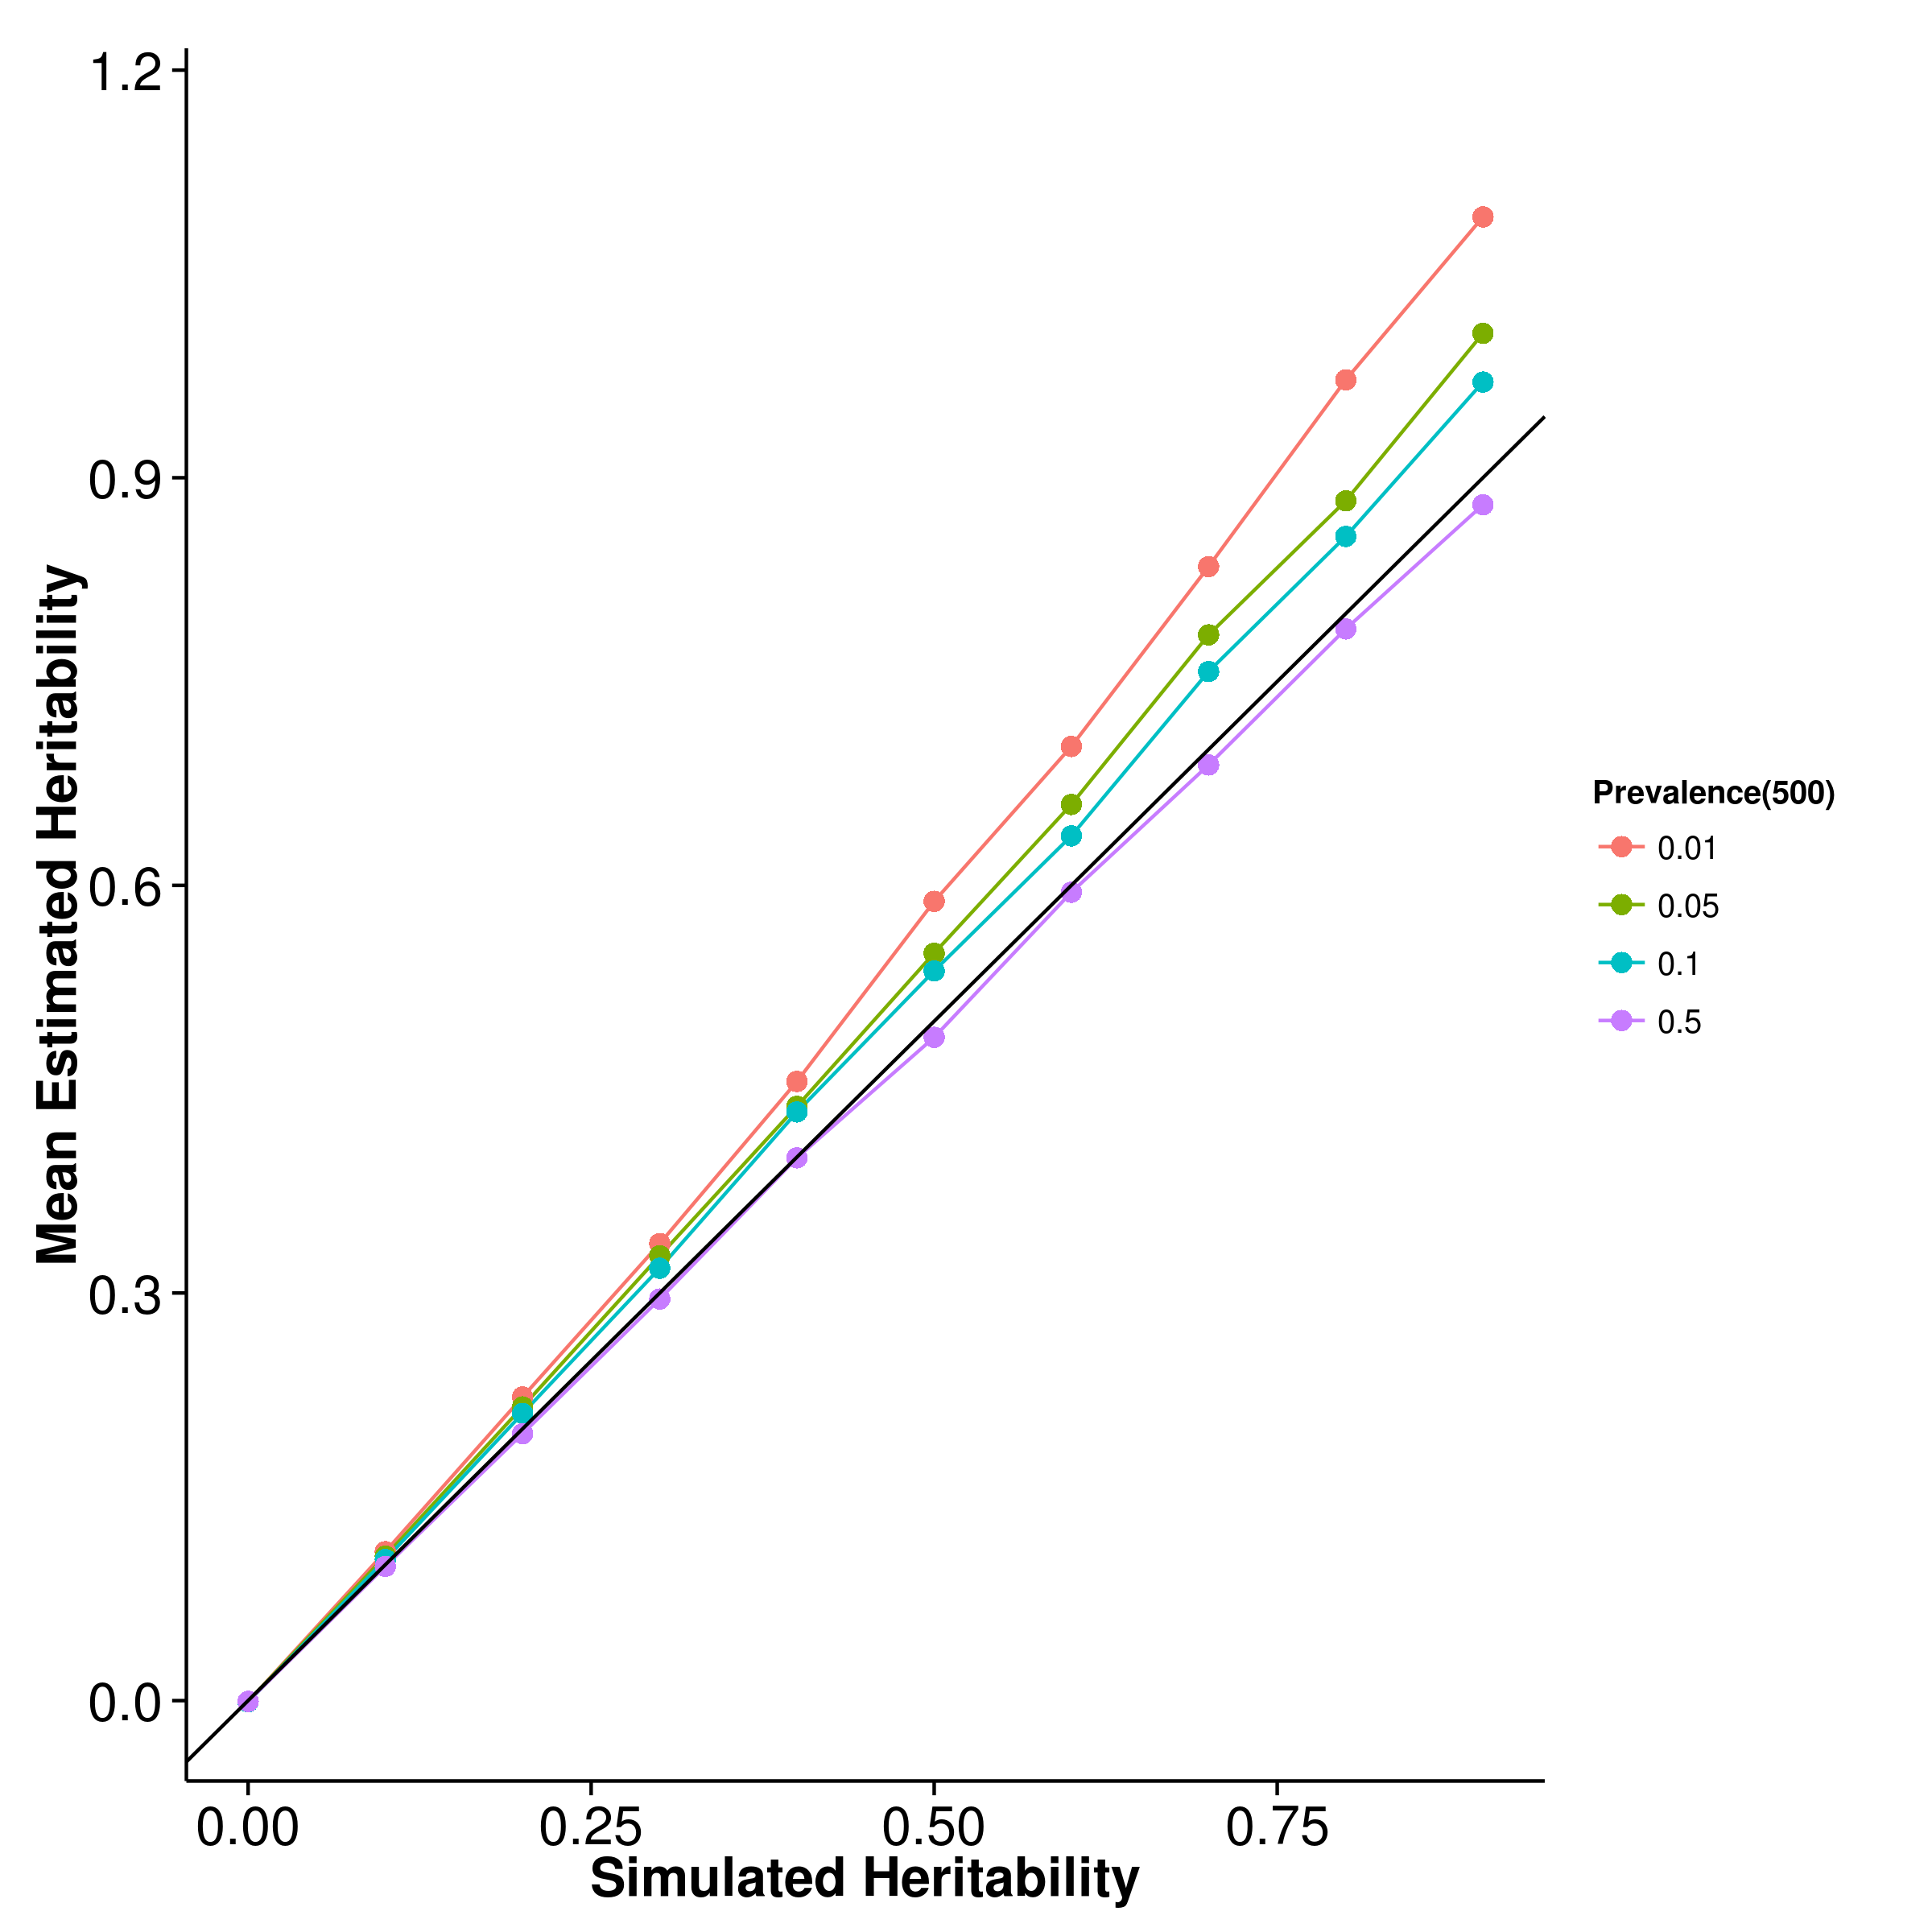
\includegraphics{figure/he_summary/cc_500c/shrek_CC_Rand_mean.png}}
				\label{fig:shrekCC500RandMean}
			}
			\subfloat[GCTA]{
				\scalebox{.4}{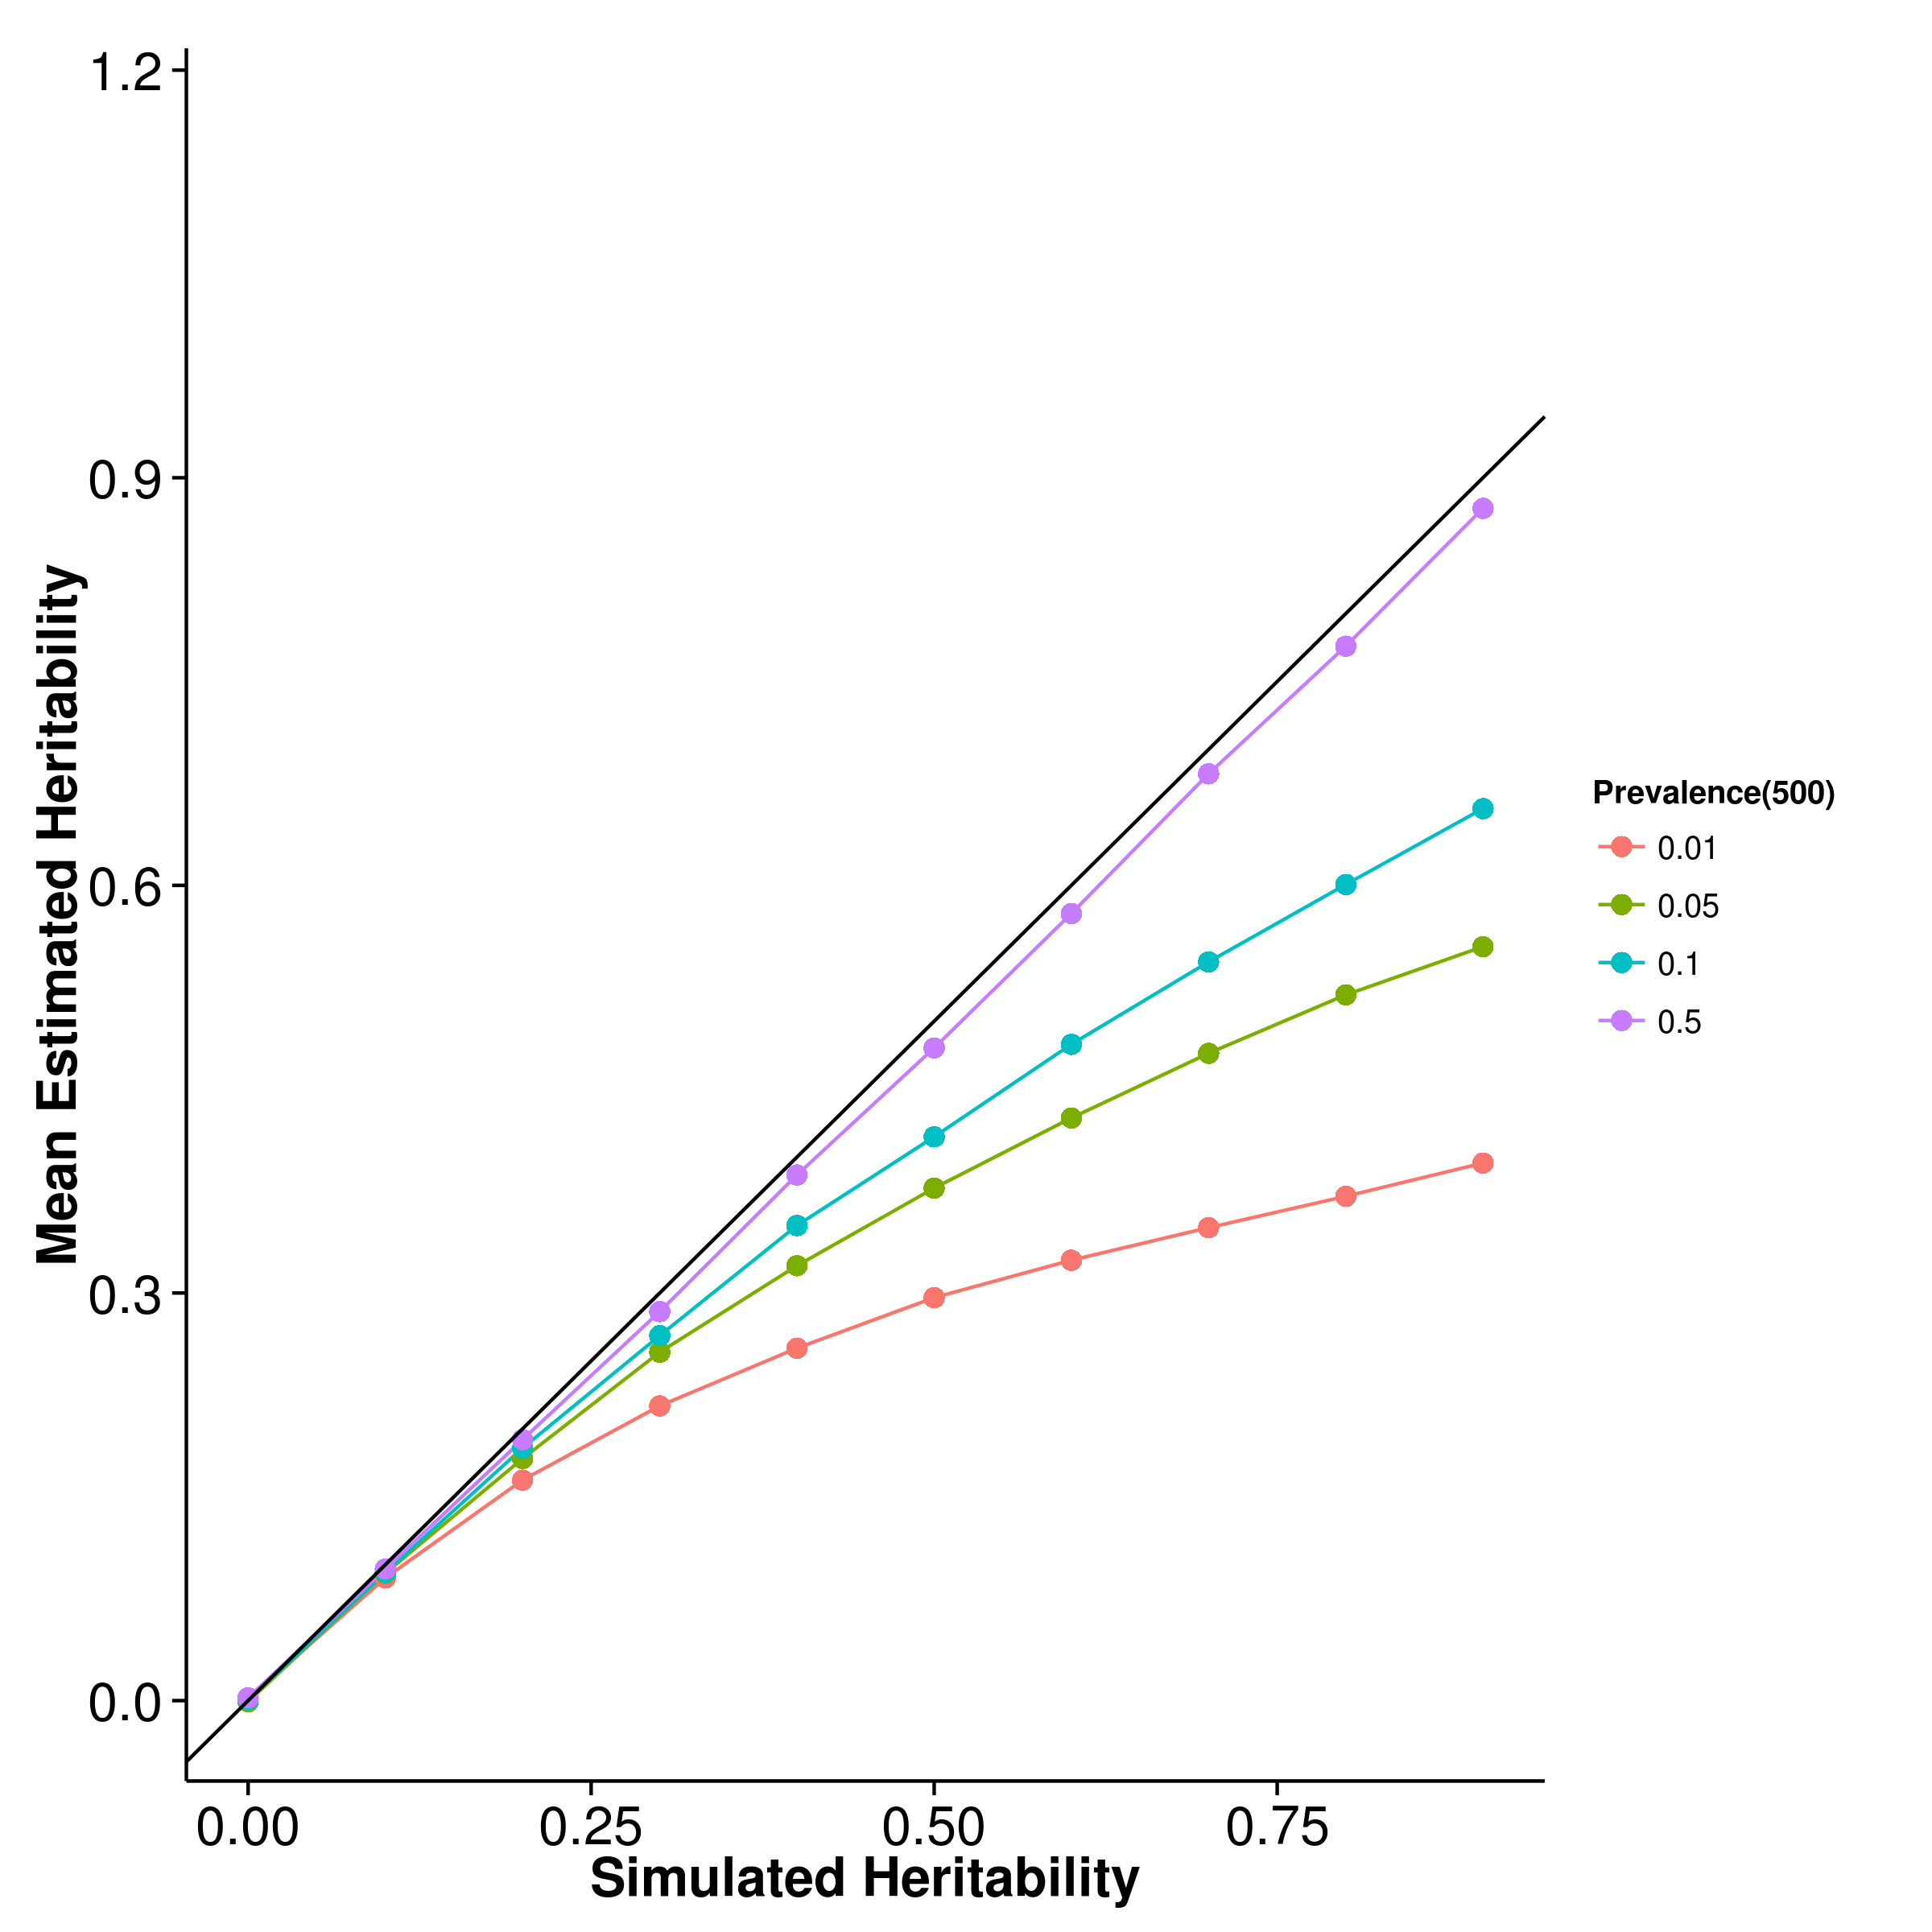
\includegraphics{figure/he_summary/cc_500c/gcta_CC_Rand_mean.png}}
				\label{fig:gctaCC500RandMean}
			}\\
			\subfloat[LDSC with fix intercept]{
				\scalebox{.4}{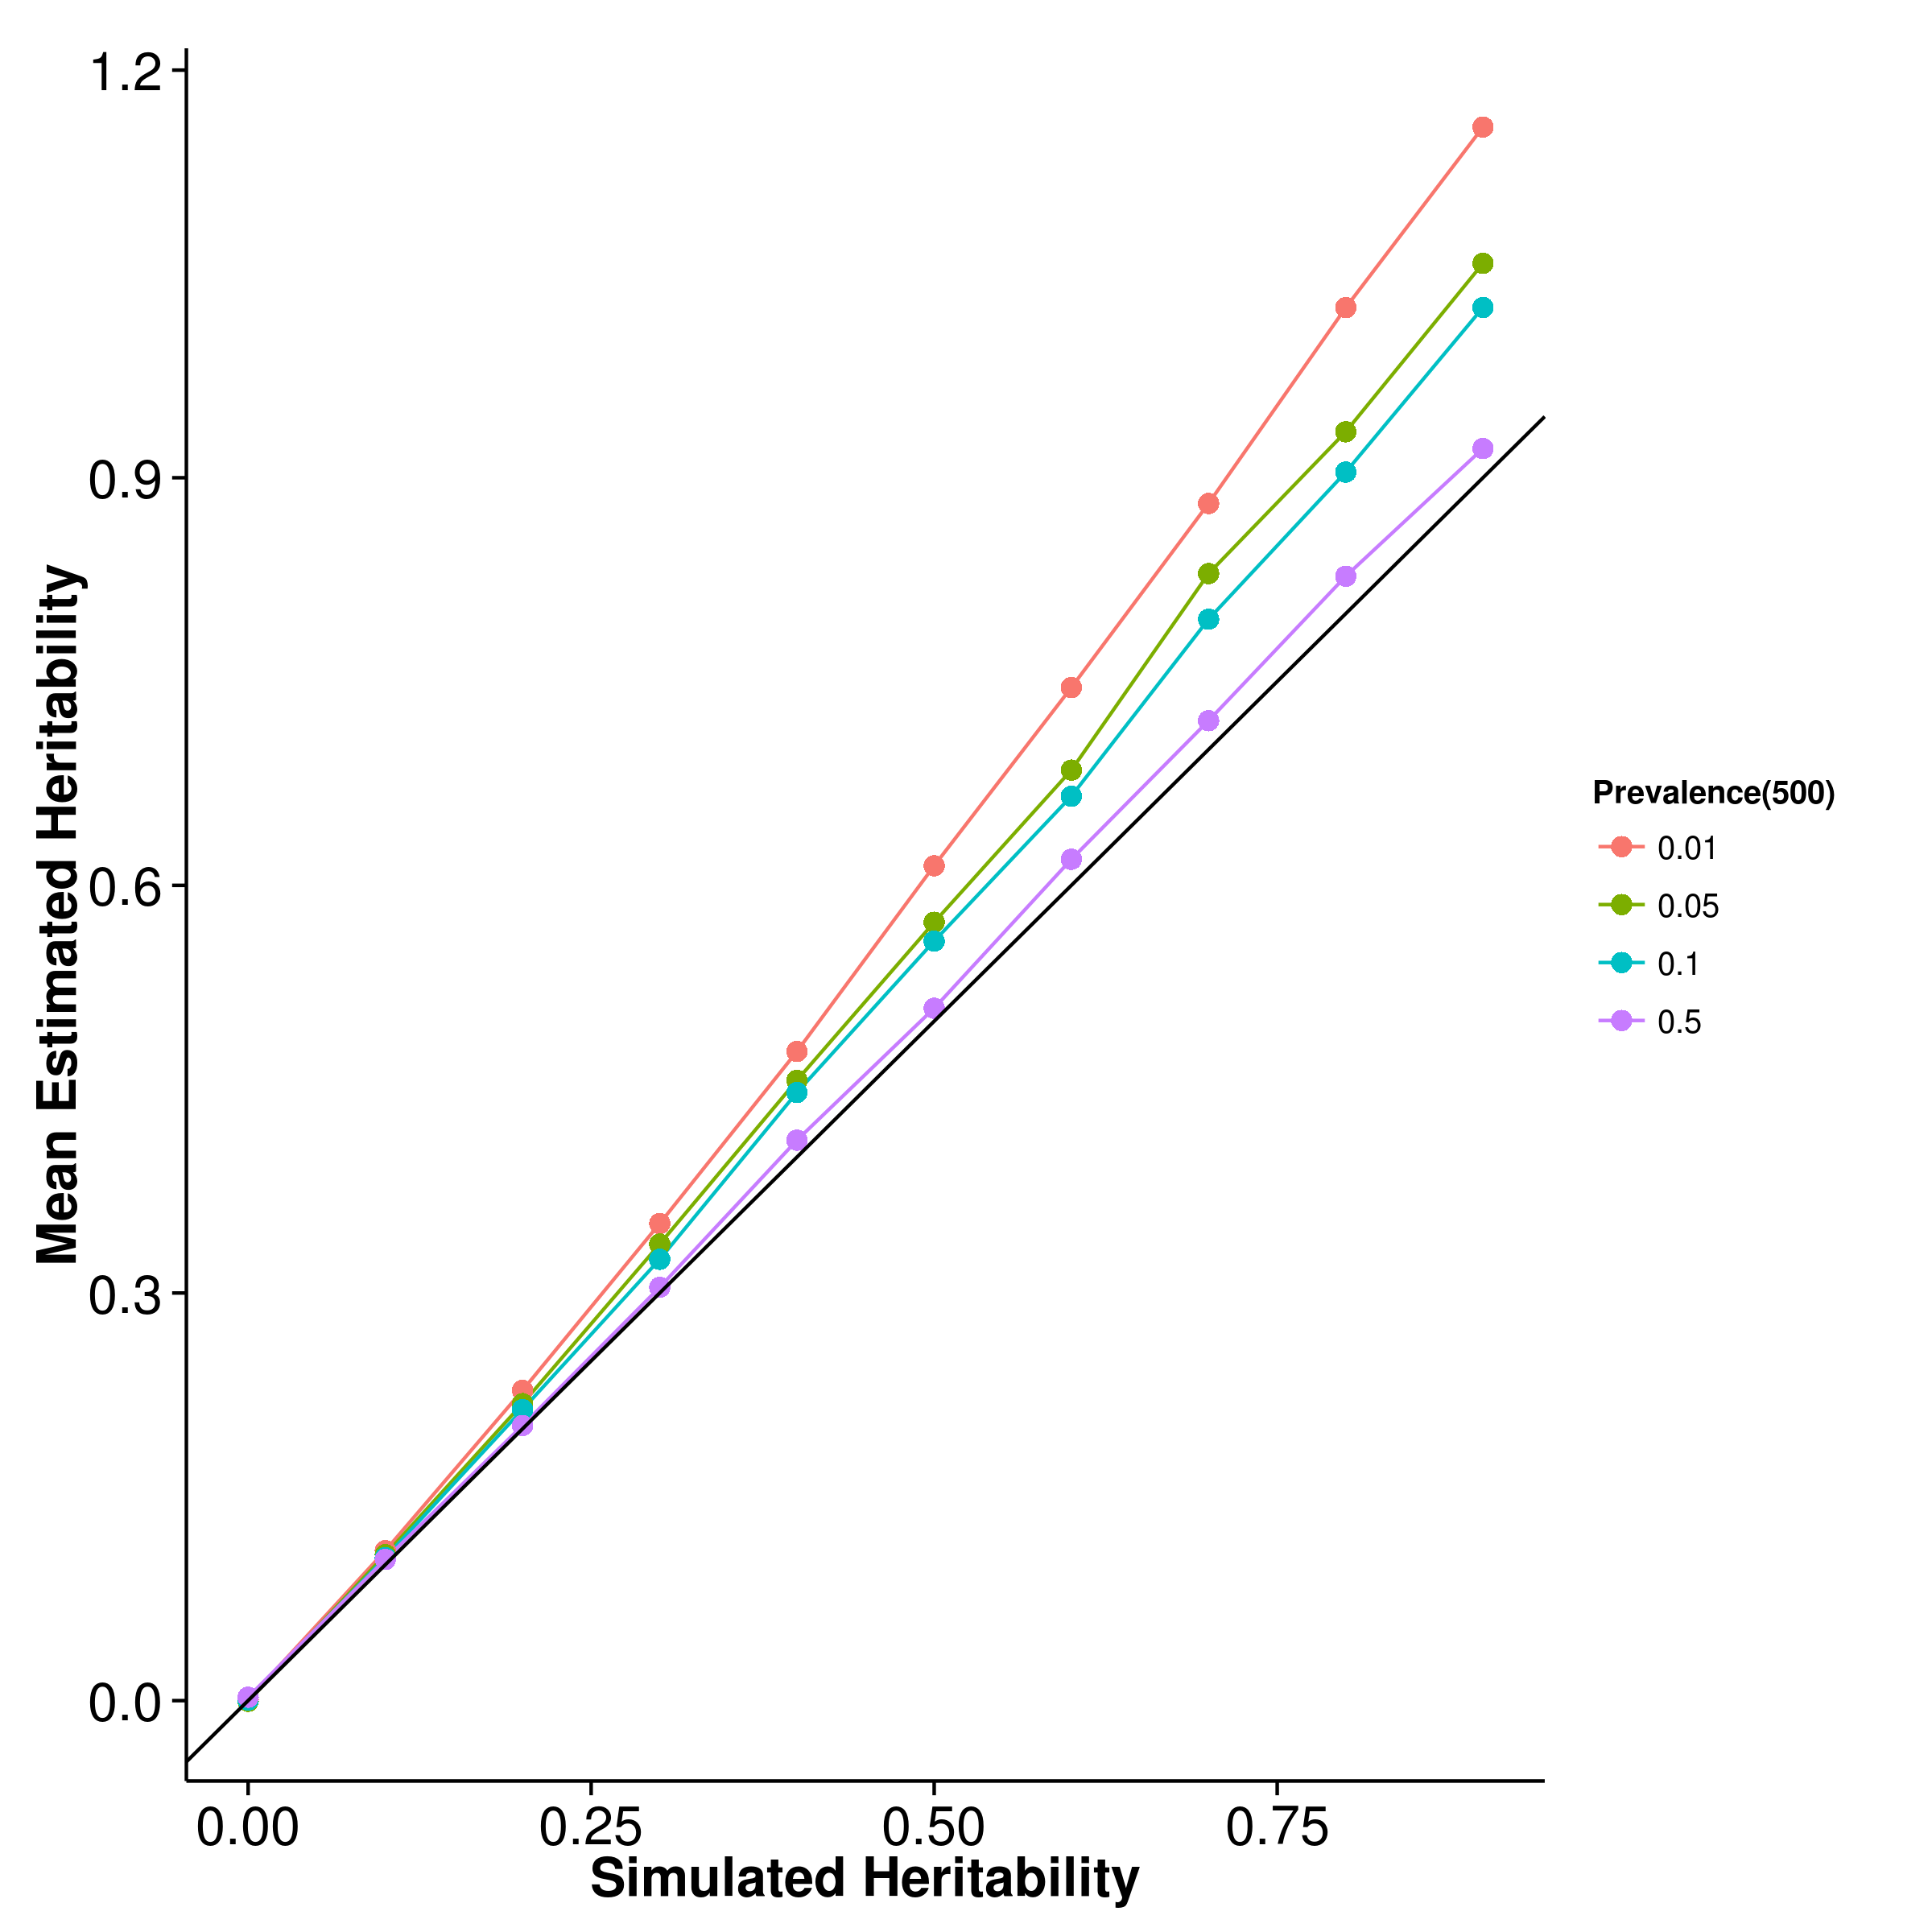
\includegraphics{figure/he_summary/cc_500c/ldsc_CC_Rand_mean.png}}
				\label{fig:ldscCC500RandMean}
			}
			\subfloat[LDSC with intercept estimation]{
				
				\scalebox{.4}{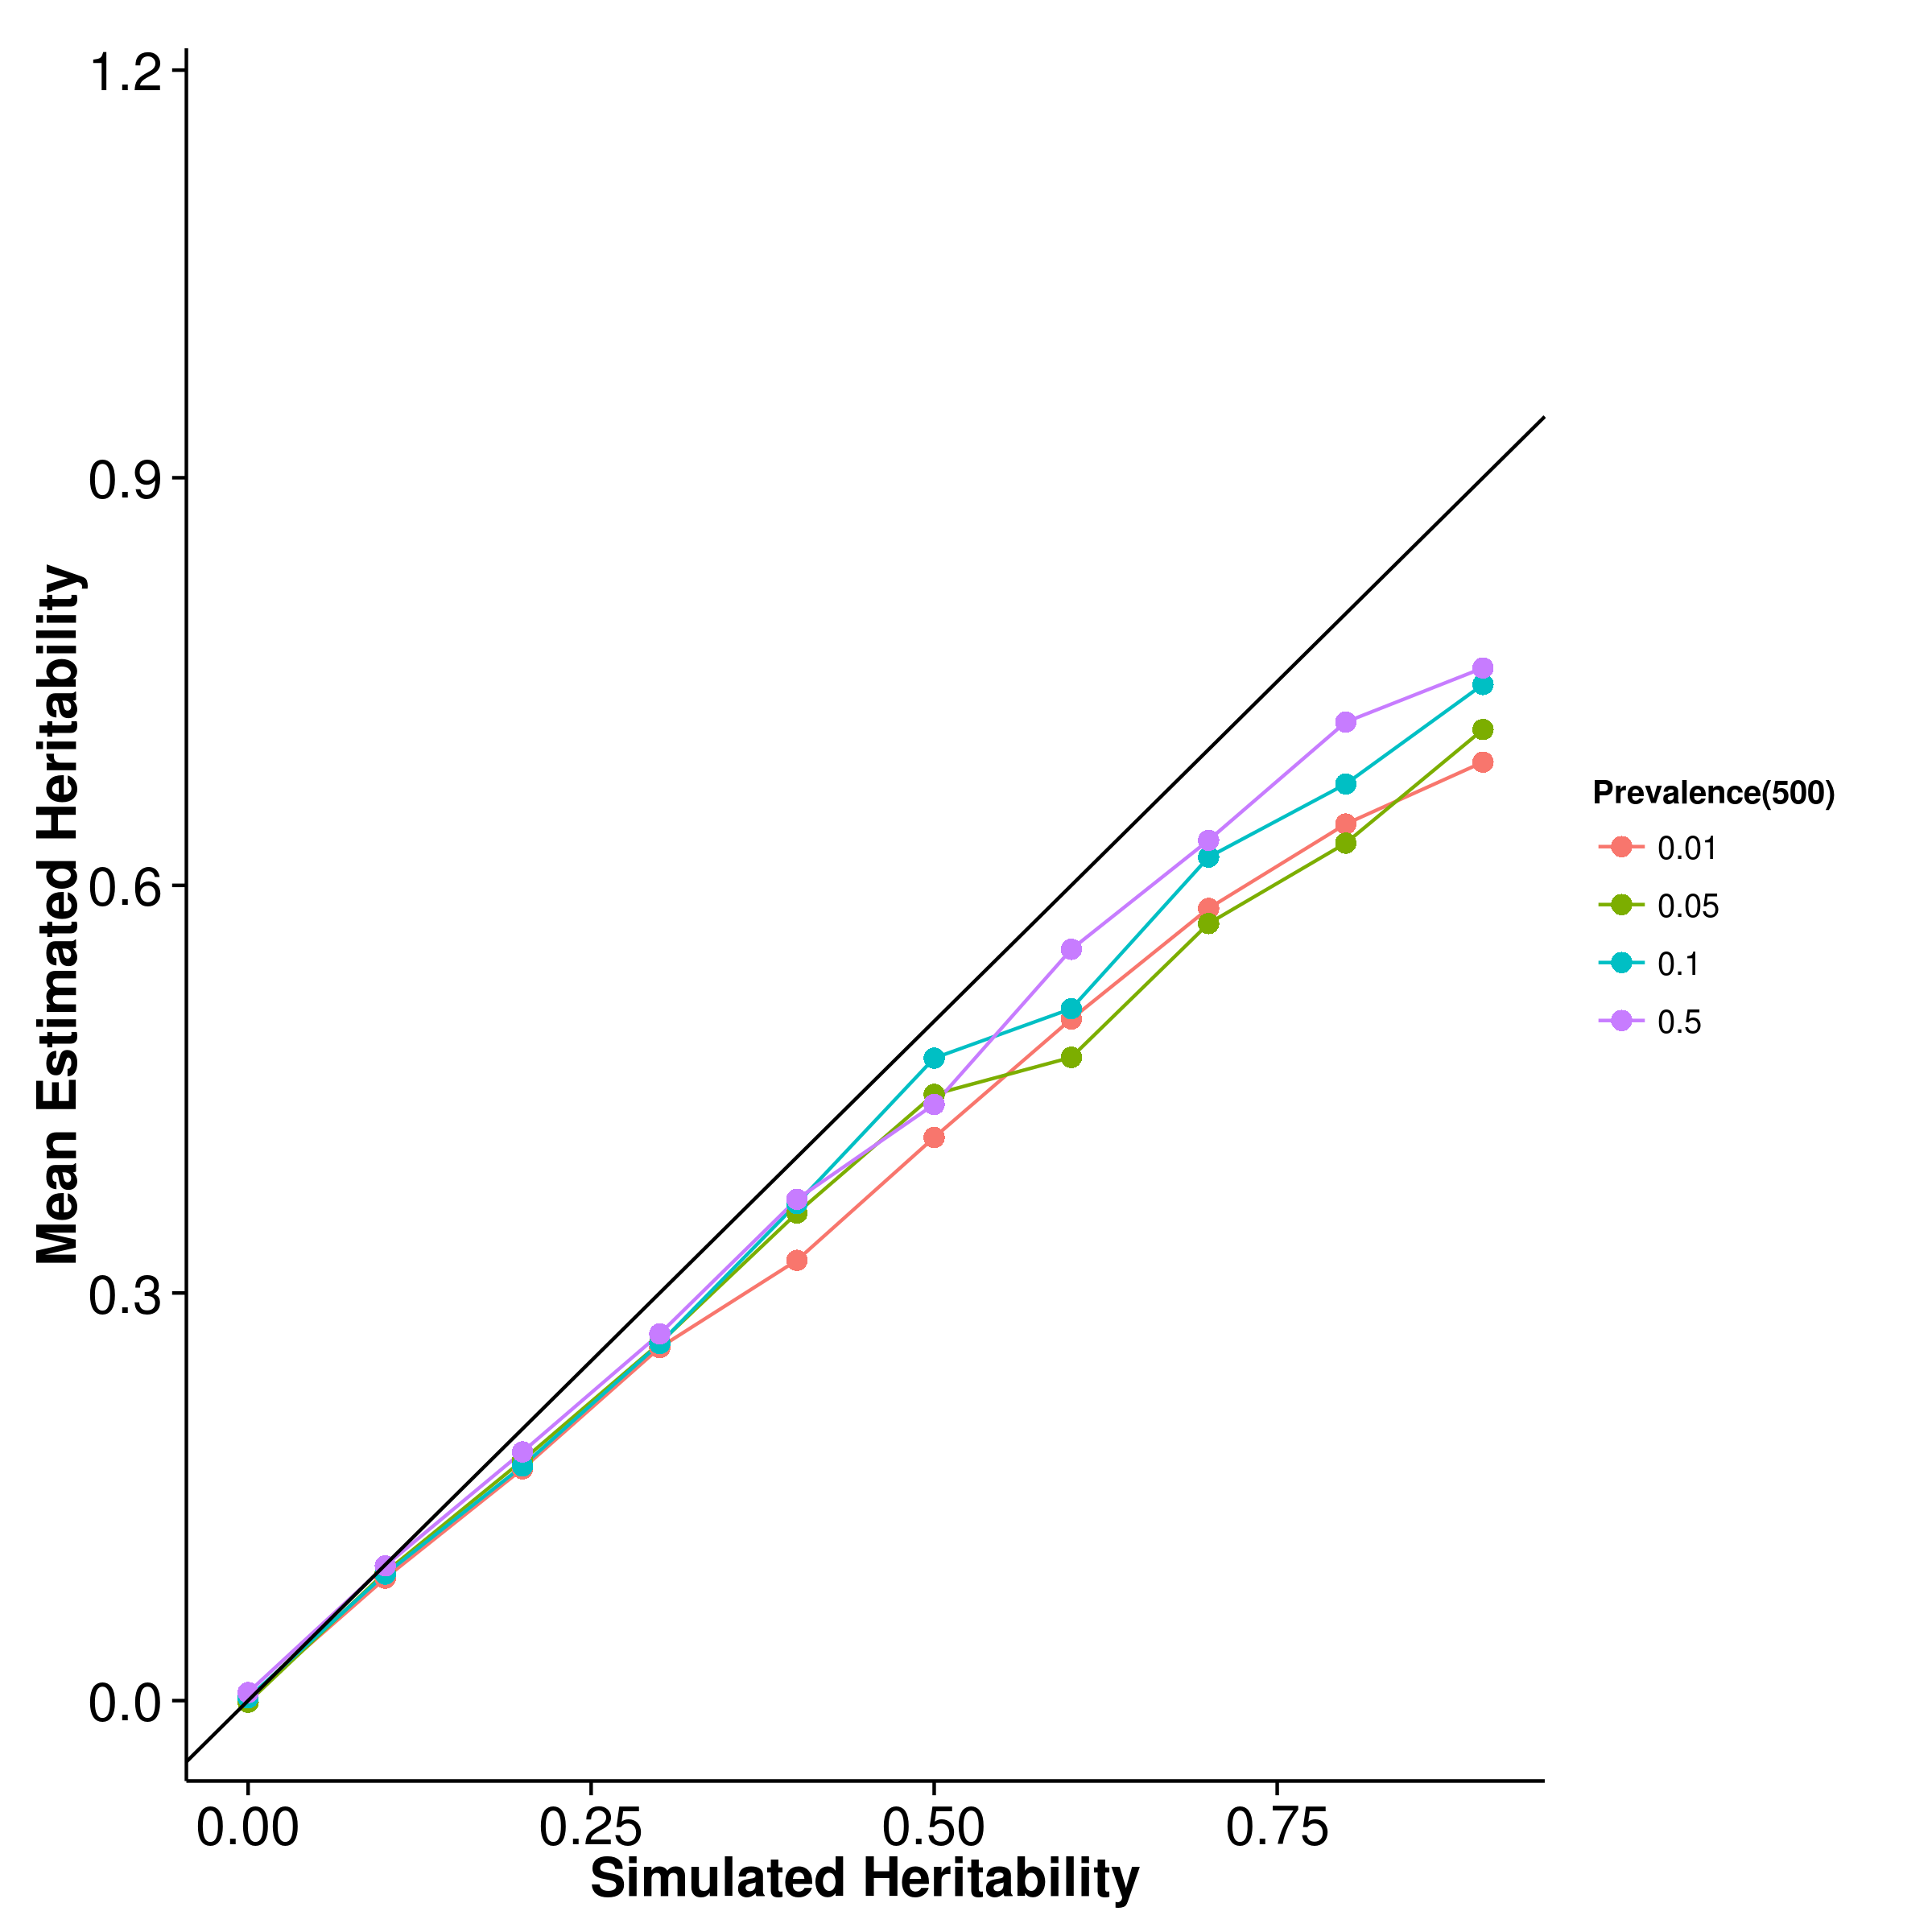
\includegraphics{figure/he_summary/cc_500c/ldscIn_CC_Rand_mean.png}}
				\label{fig:ldscInCC500RandMean}
			}
			\caption[Mean of Case Control Simulation Results (500 Causal)]
			{Mean of results from case control simulation with random effect size simulation with 500 causal \glspl{SNP}.
				Again, a clear pattern of underestimation was observed for \gls{gcta} and \gls{ldsc} with intercept estimation whereas estimations from \gls{shrek} and \gls{ldsc} with fixed intercepts tends to be upwardly biased, with the magnitude of bias increases as the population prevalence decreases.
				} 
			\label{fig:CC500RandMean}
		\end{figure}
		
		\begin{figure}
			\centering
			\subfloat[SHREK]{
				\scalebox{.4}{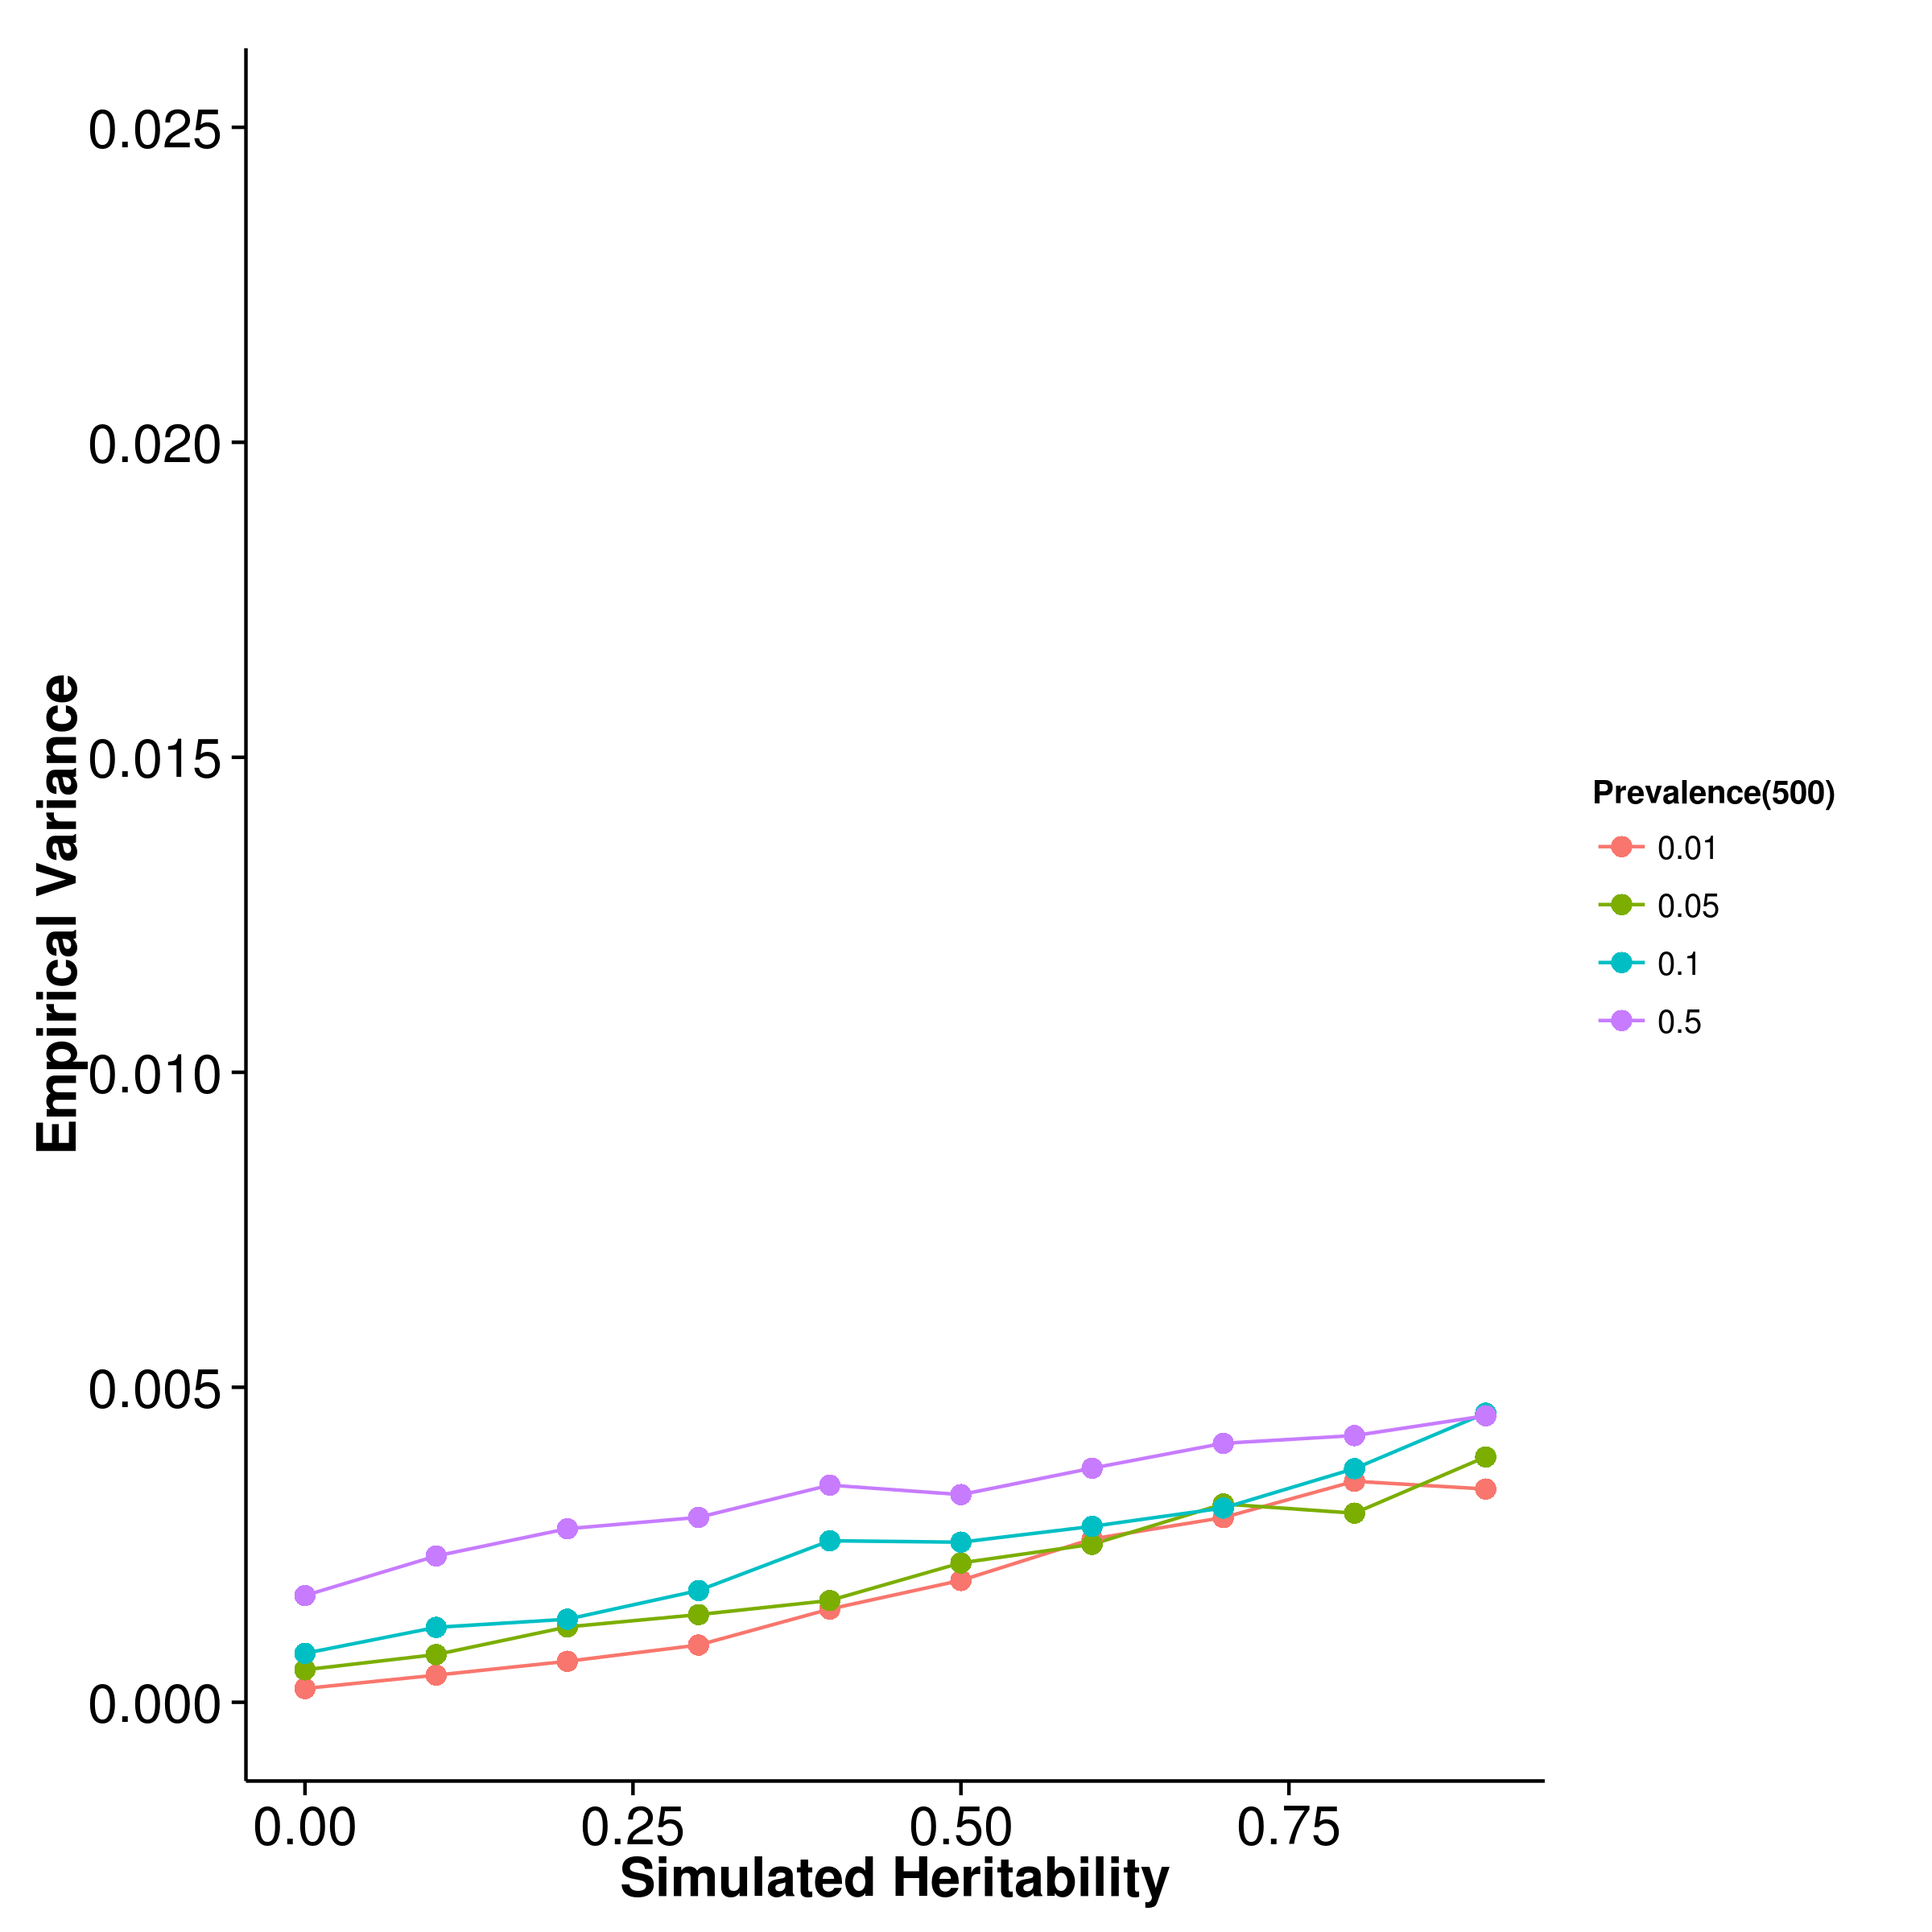
\includegraphics{figure/he_summary/cc_500c/shrek_CC_Rand_sd.png}}
				\label{fig:shrekCC500RandVar}
			}
			\subfloat[GCTA]{
				\scalebox{.4}{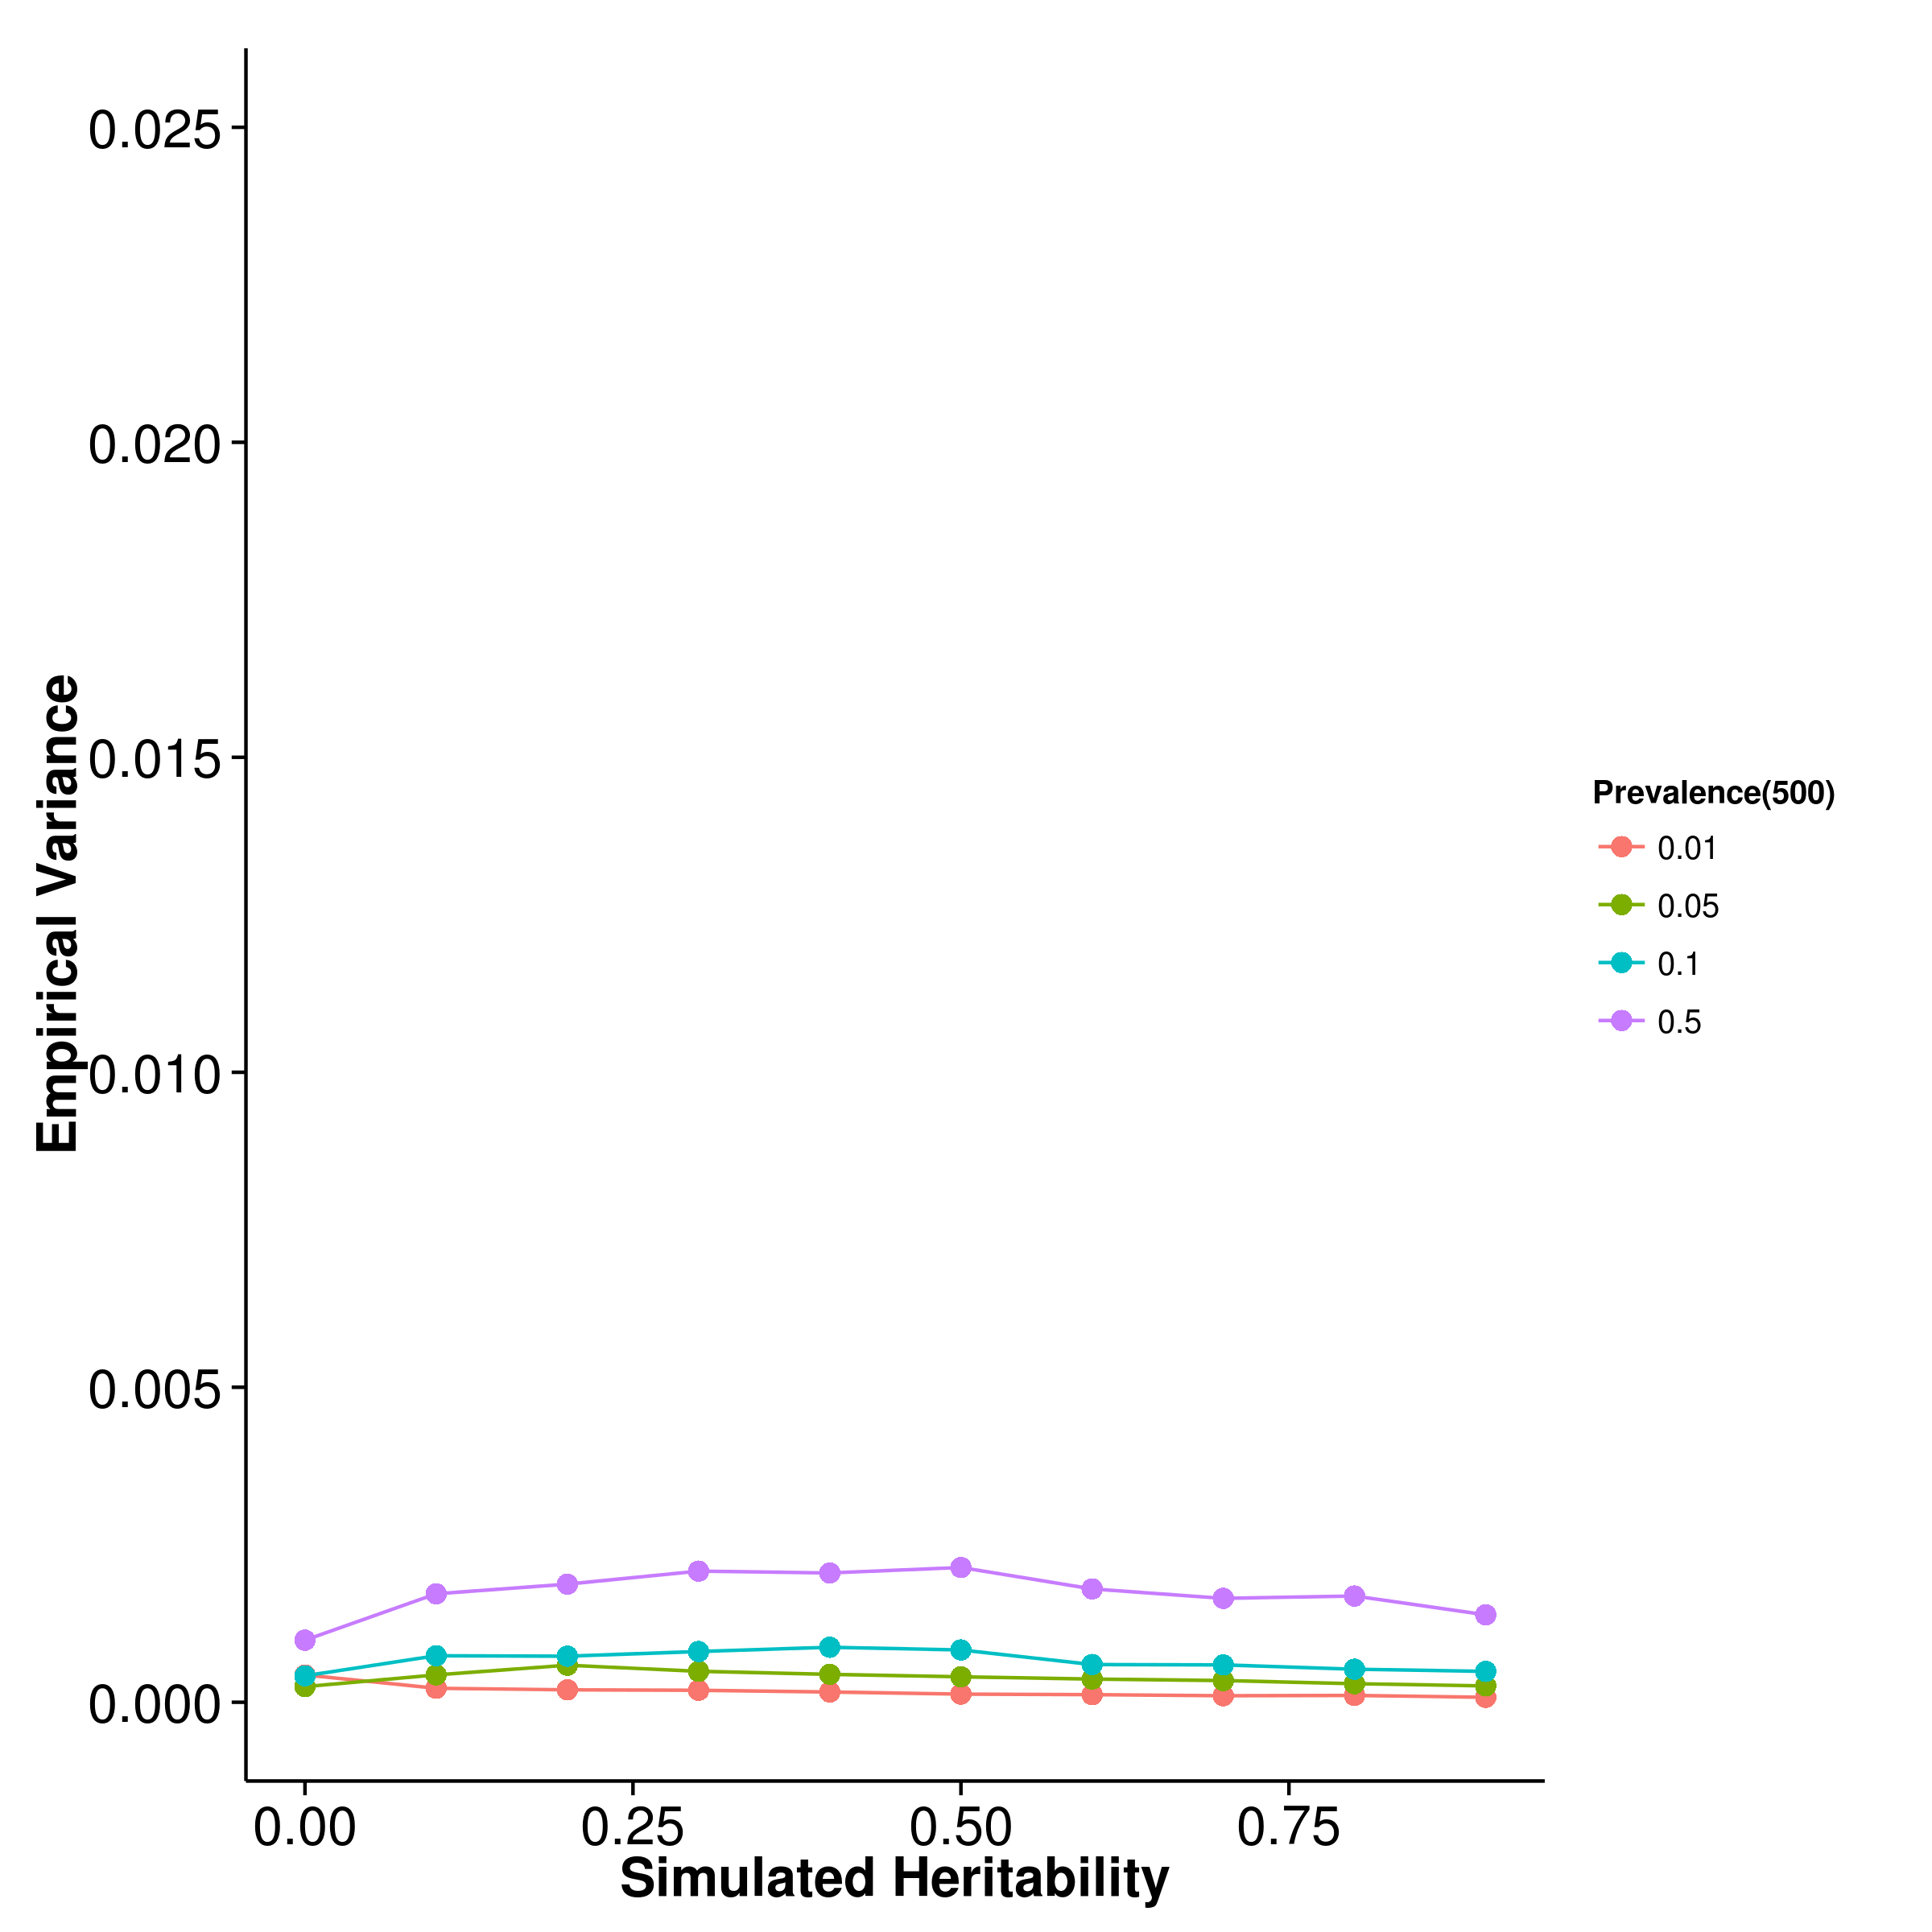
\includegraphics{figure/he_summary/cc_500c/gcta_CC_Rand_sd.png}}
				\label{fig:gctaCC500RandVar}
			}\\
			\subfloat[LDSC with fix intercept]{
				\scalebox{.4}{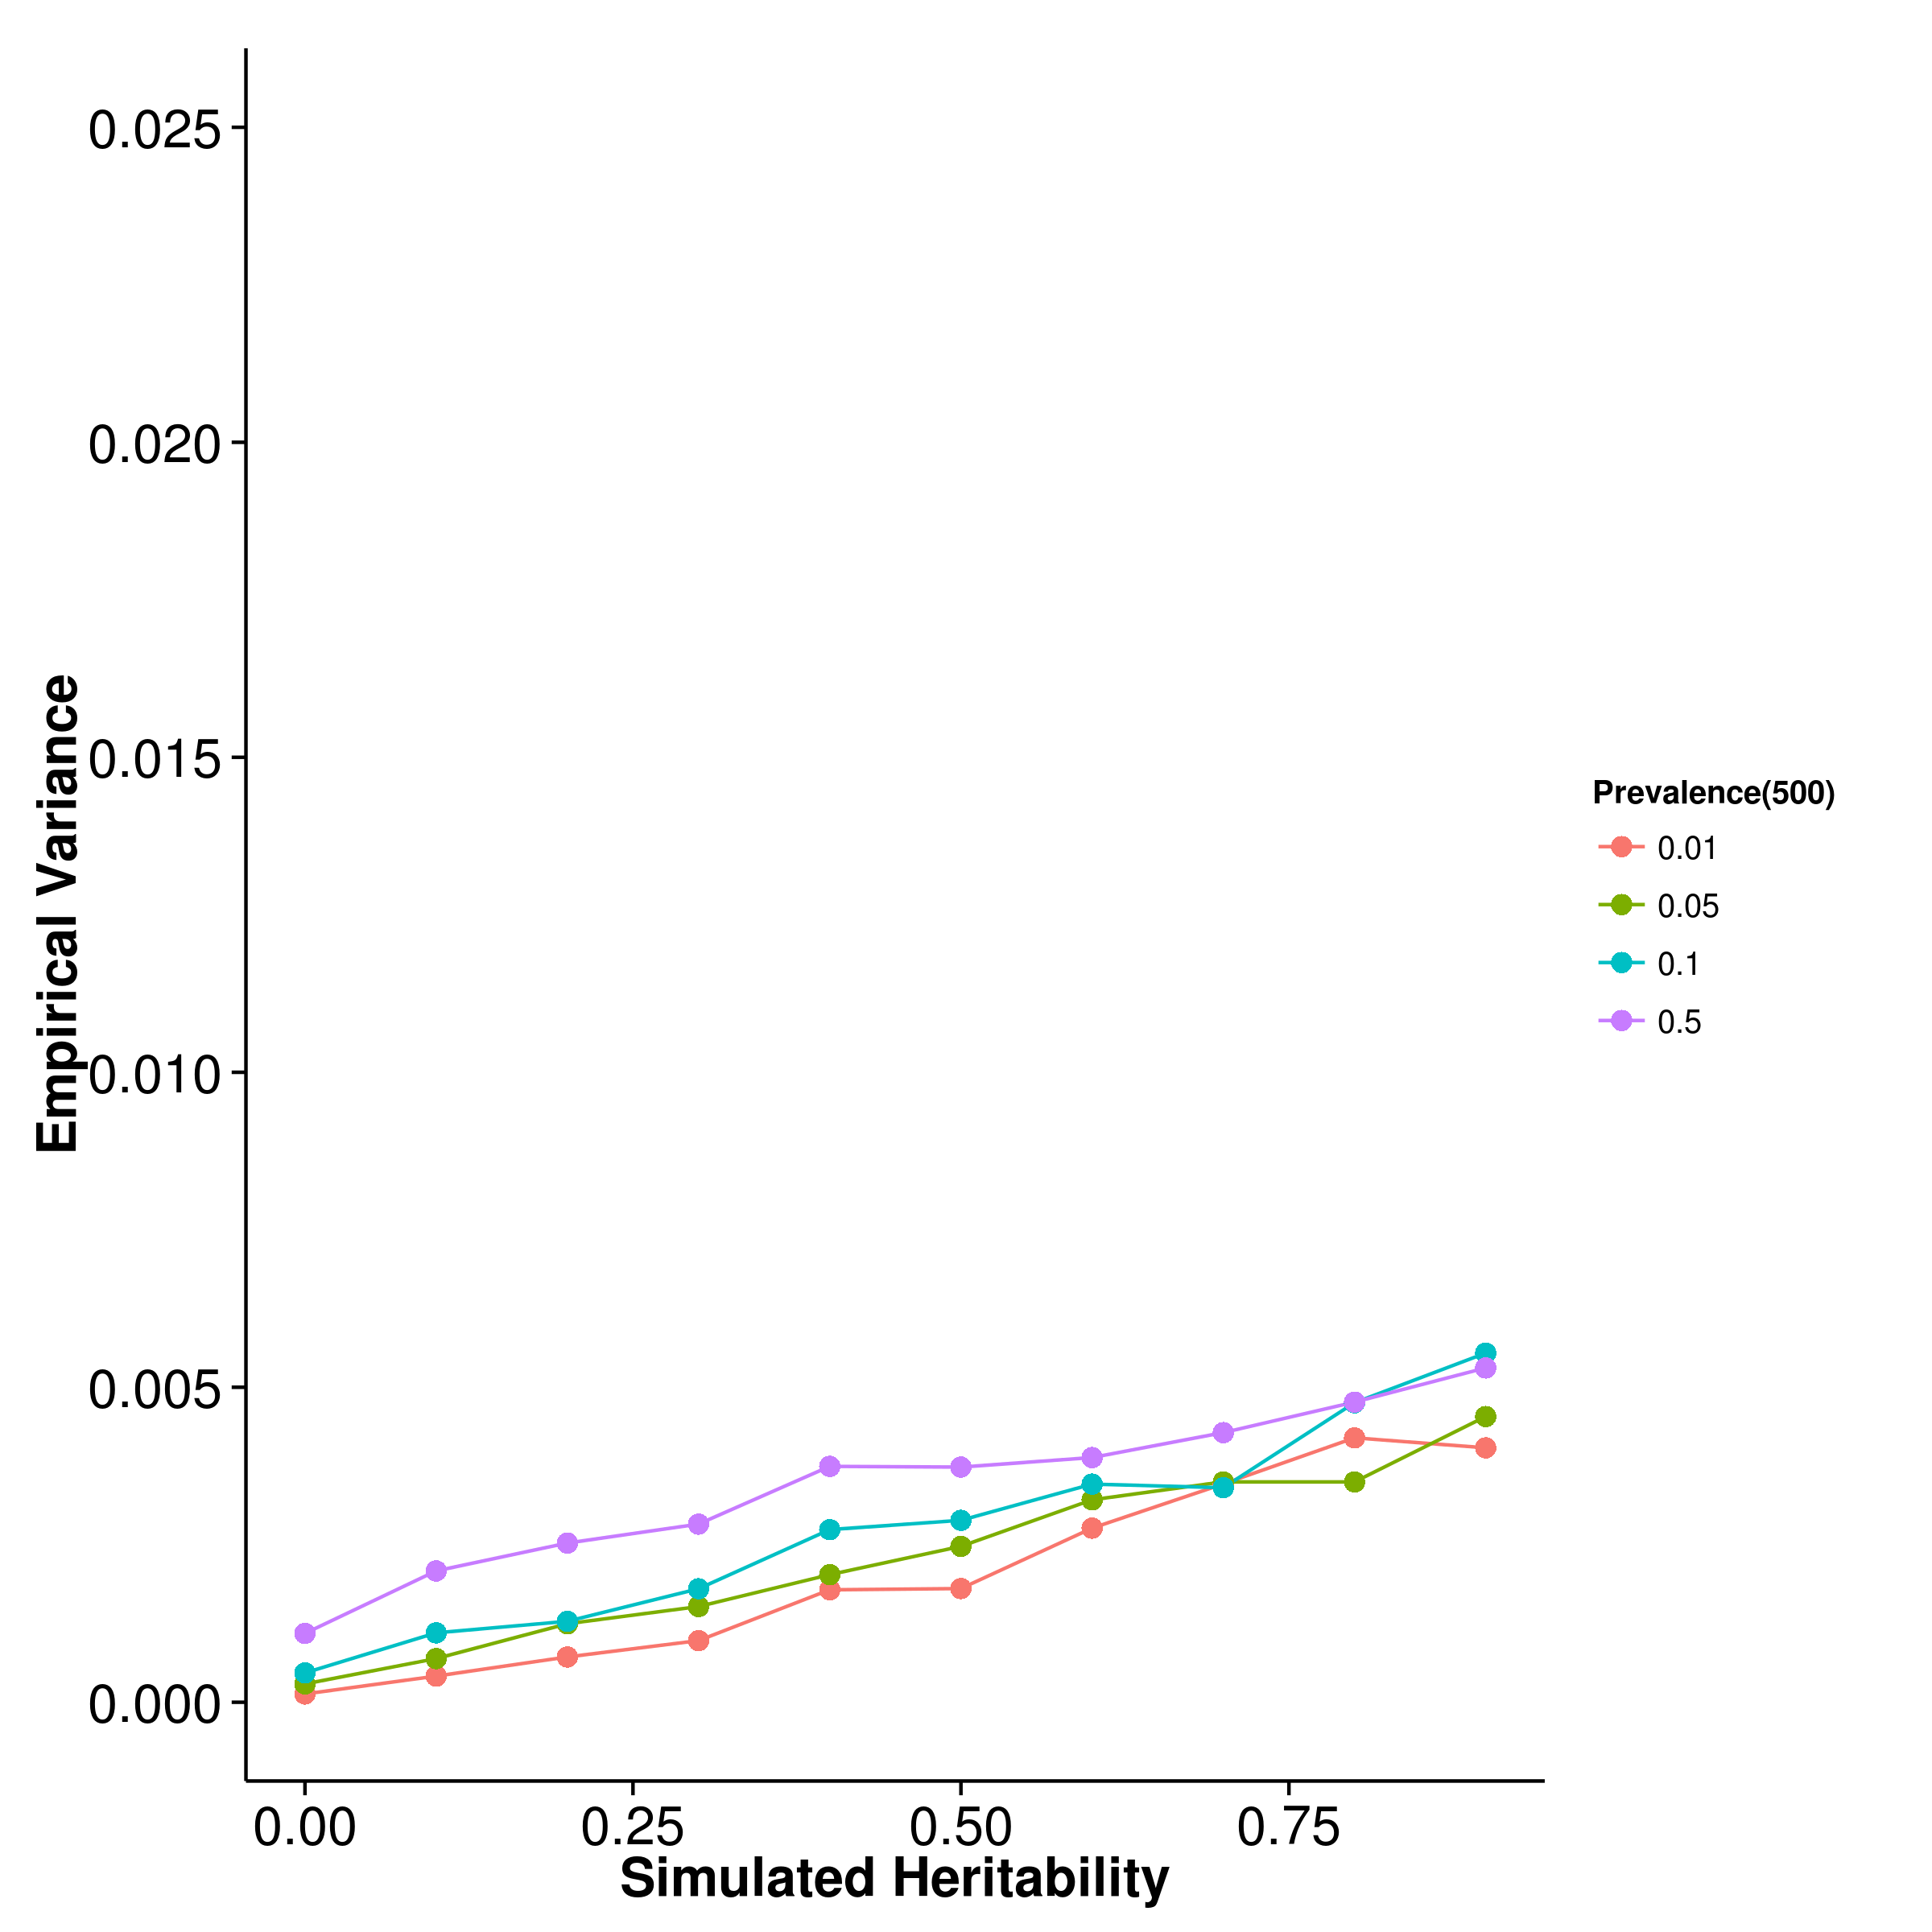
\includegraphics{figure/he_summary/cc_500c/ldsc_CC_Rand_sd.png}}
				\label{fig:ldscCC500RandVar}
			}
			\subfloat[LDSC with intercept estimation]{
				
				\scalebox{.4}{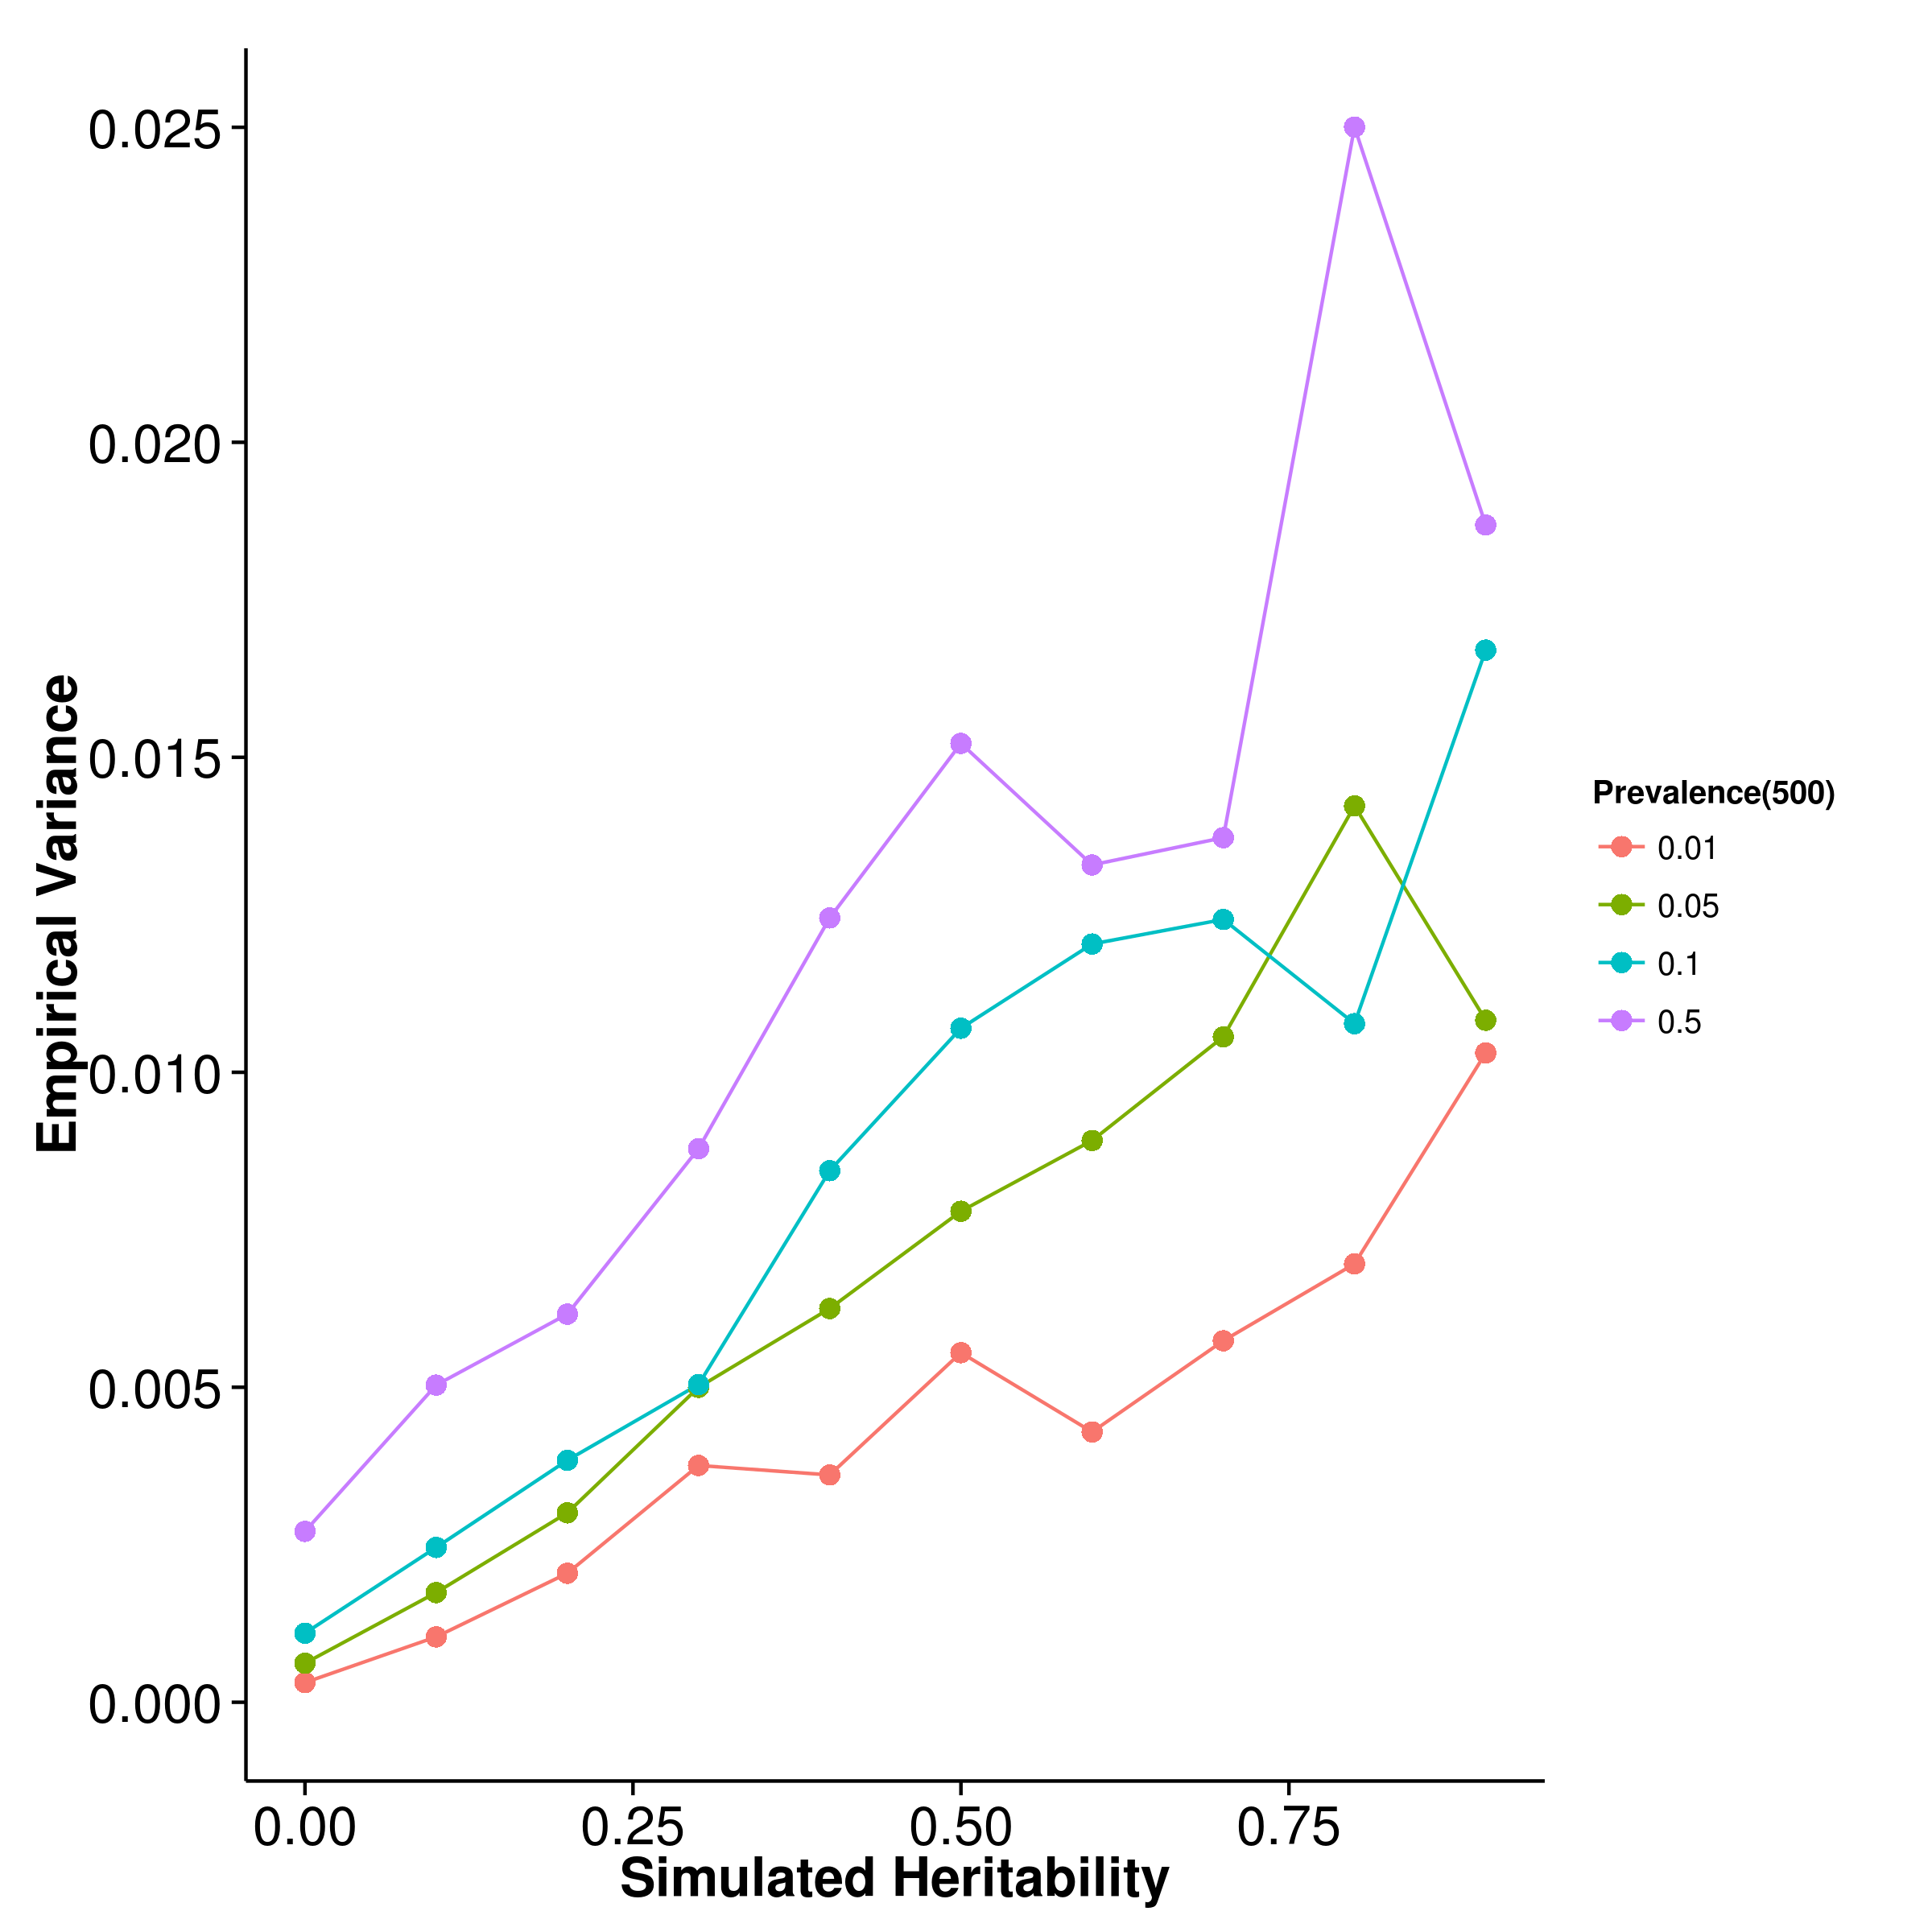
\includegraphics{figure/he_summary/cc_500c/ldscIn_CC_Rand_sd.png}}
				\label{fig:ldscInCC500RandVar}
			}
			\caption[Variance of Case Control Simulation Results (500 Causal)]
			{Variance of results from case control simulation with random effect size simulation with 500 causal \glspl{SNP}.
				As the number of causal \glspl{SNP} increased to 500, the empirical variance of \gls{shrek} and \gls{ldsc} with fixed intercept converges. 
				However, the empirical variance of \gls{ldsc} with intercept estimations remains high. 
			} 
			\label{fig:CC500RandVar}
		\end{figure}
		
		
		\begin{figure}
			\centering
			\subfloat[SHREK]{
				\scalebox{.4}{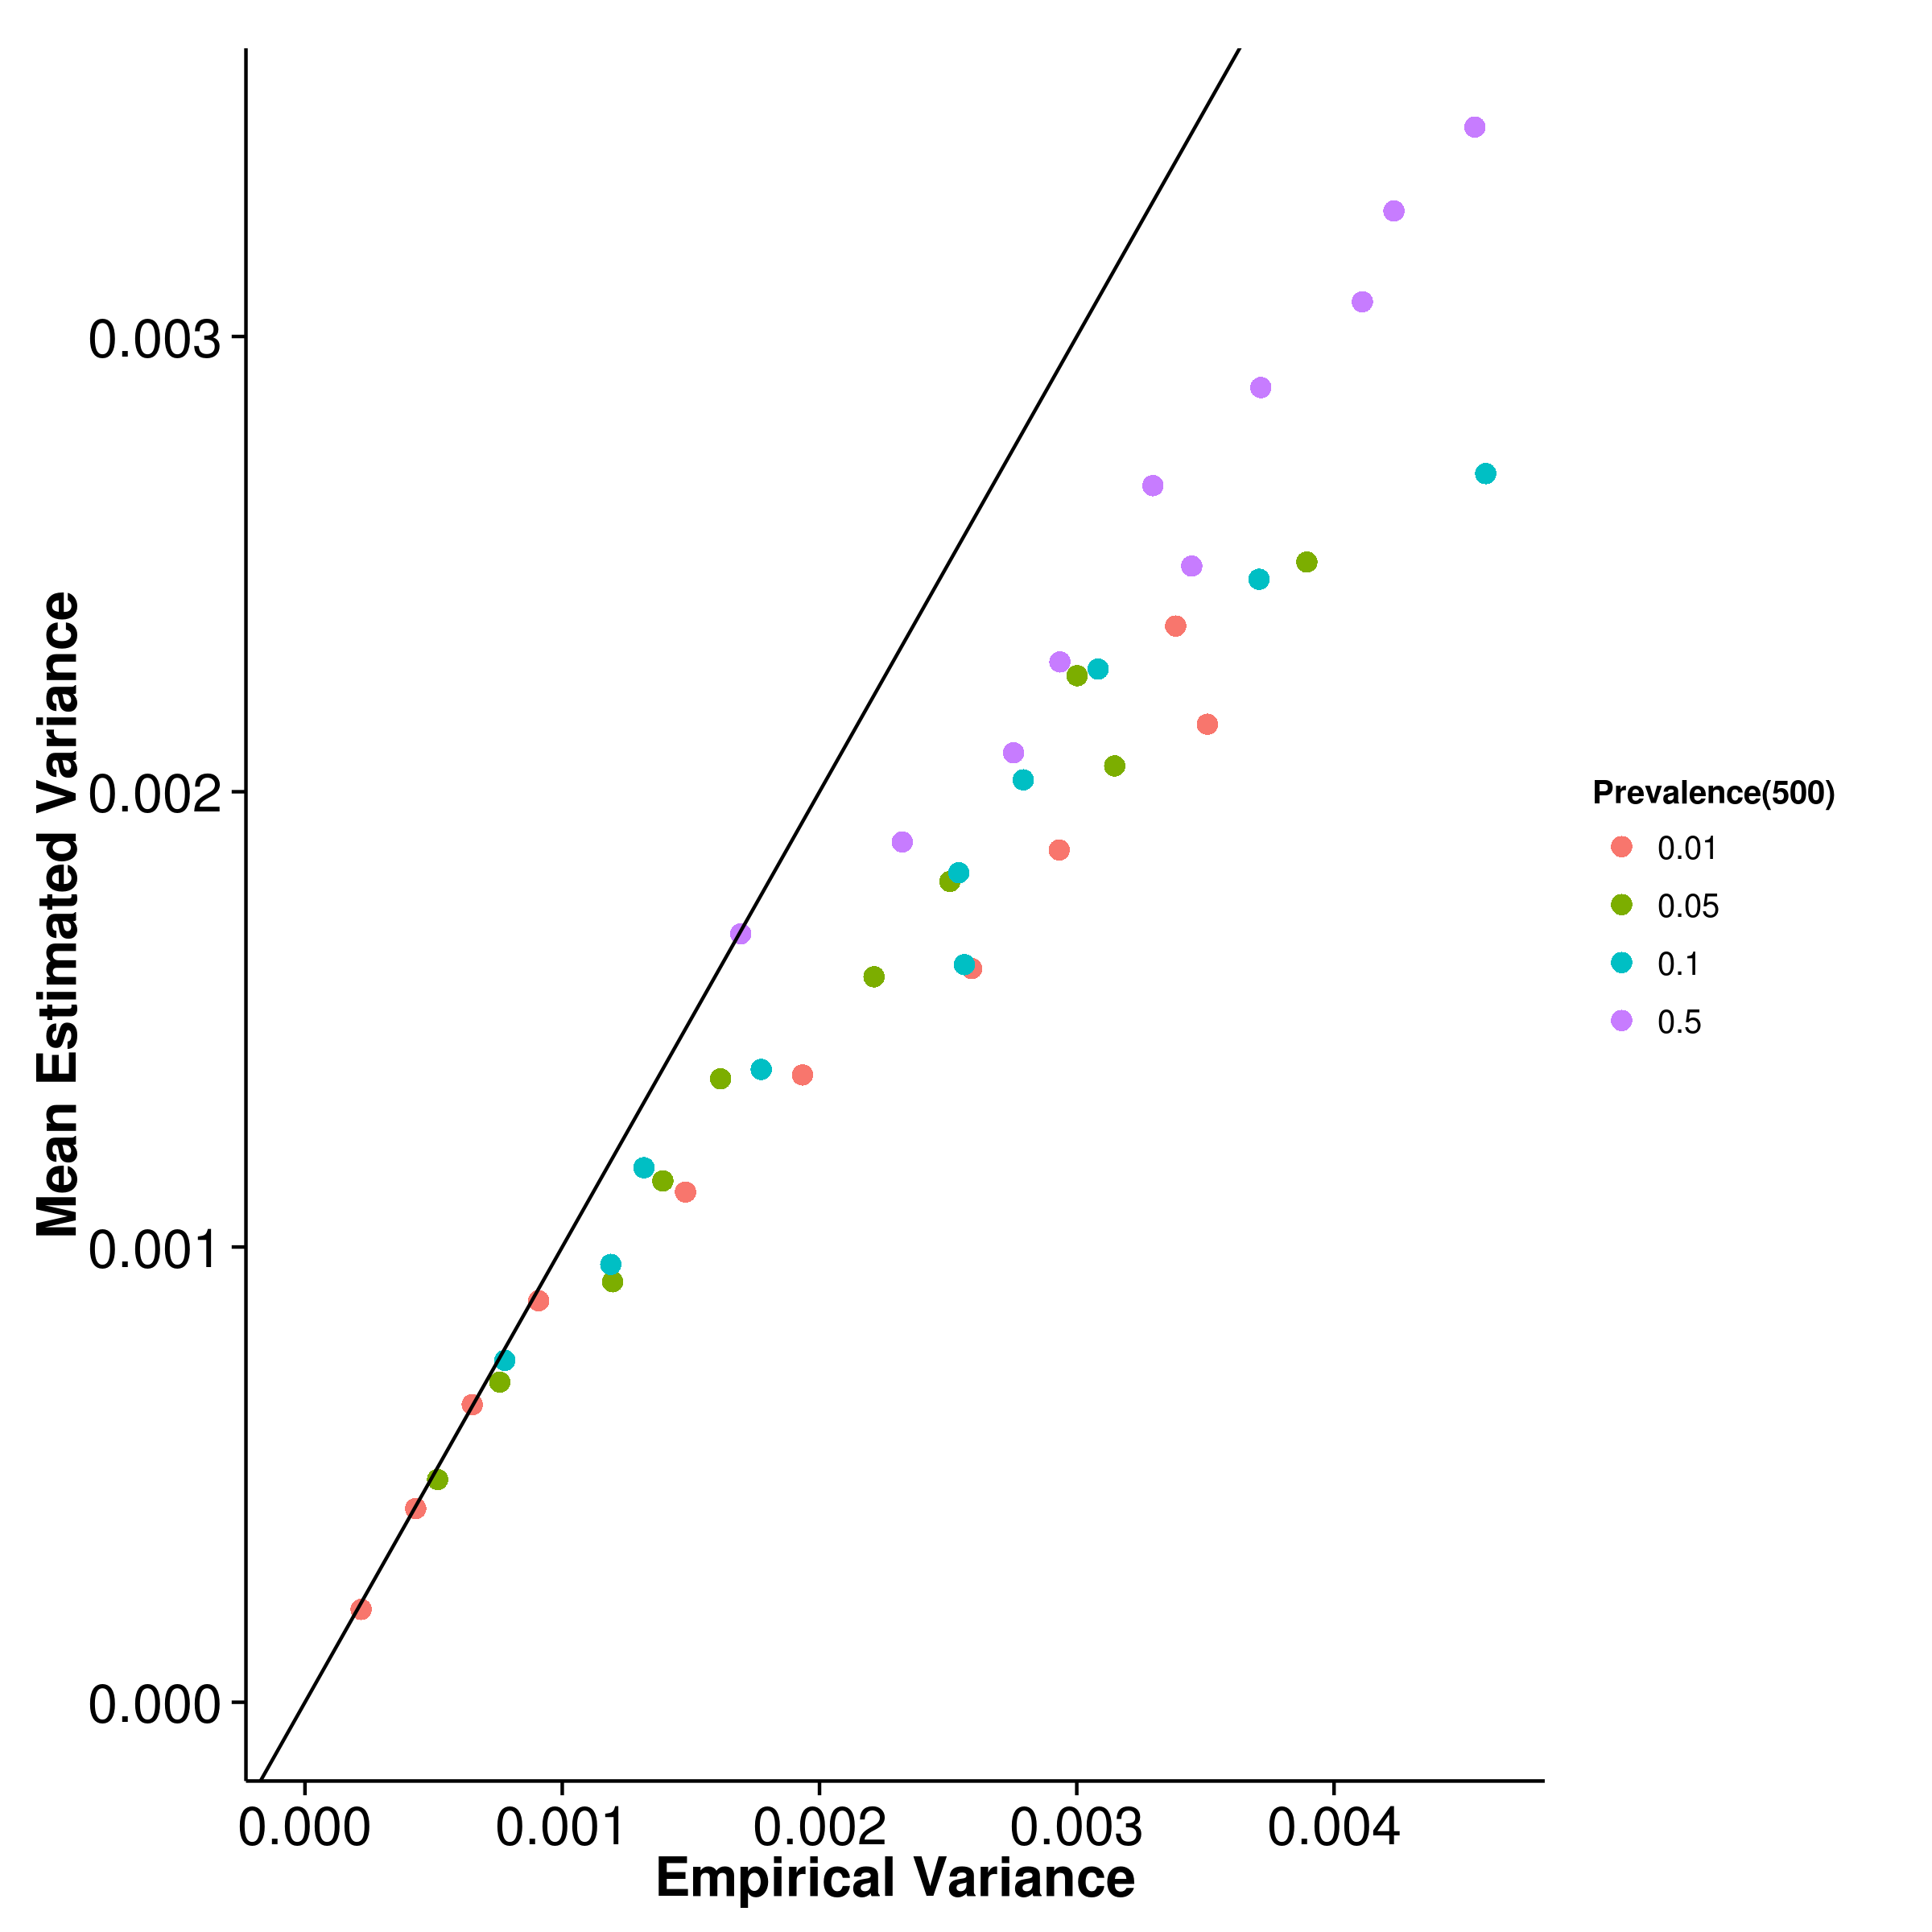
\includegraphics{figure/he_summary/cc_500c/shrek_CC_Rand_sdCom.png}}
				\label{fig:shrekCC500RandVarCom}
			}
			\subfloat[GCTA]{
				\scalebox{.4}{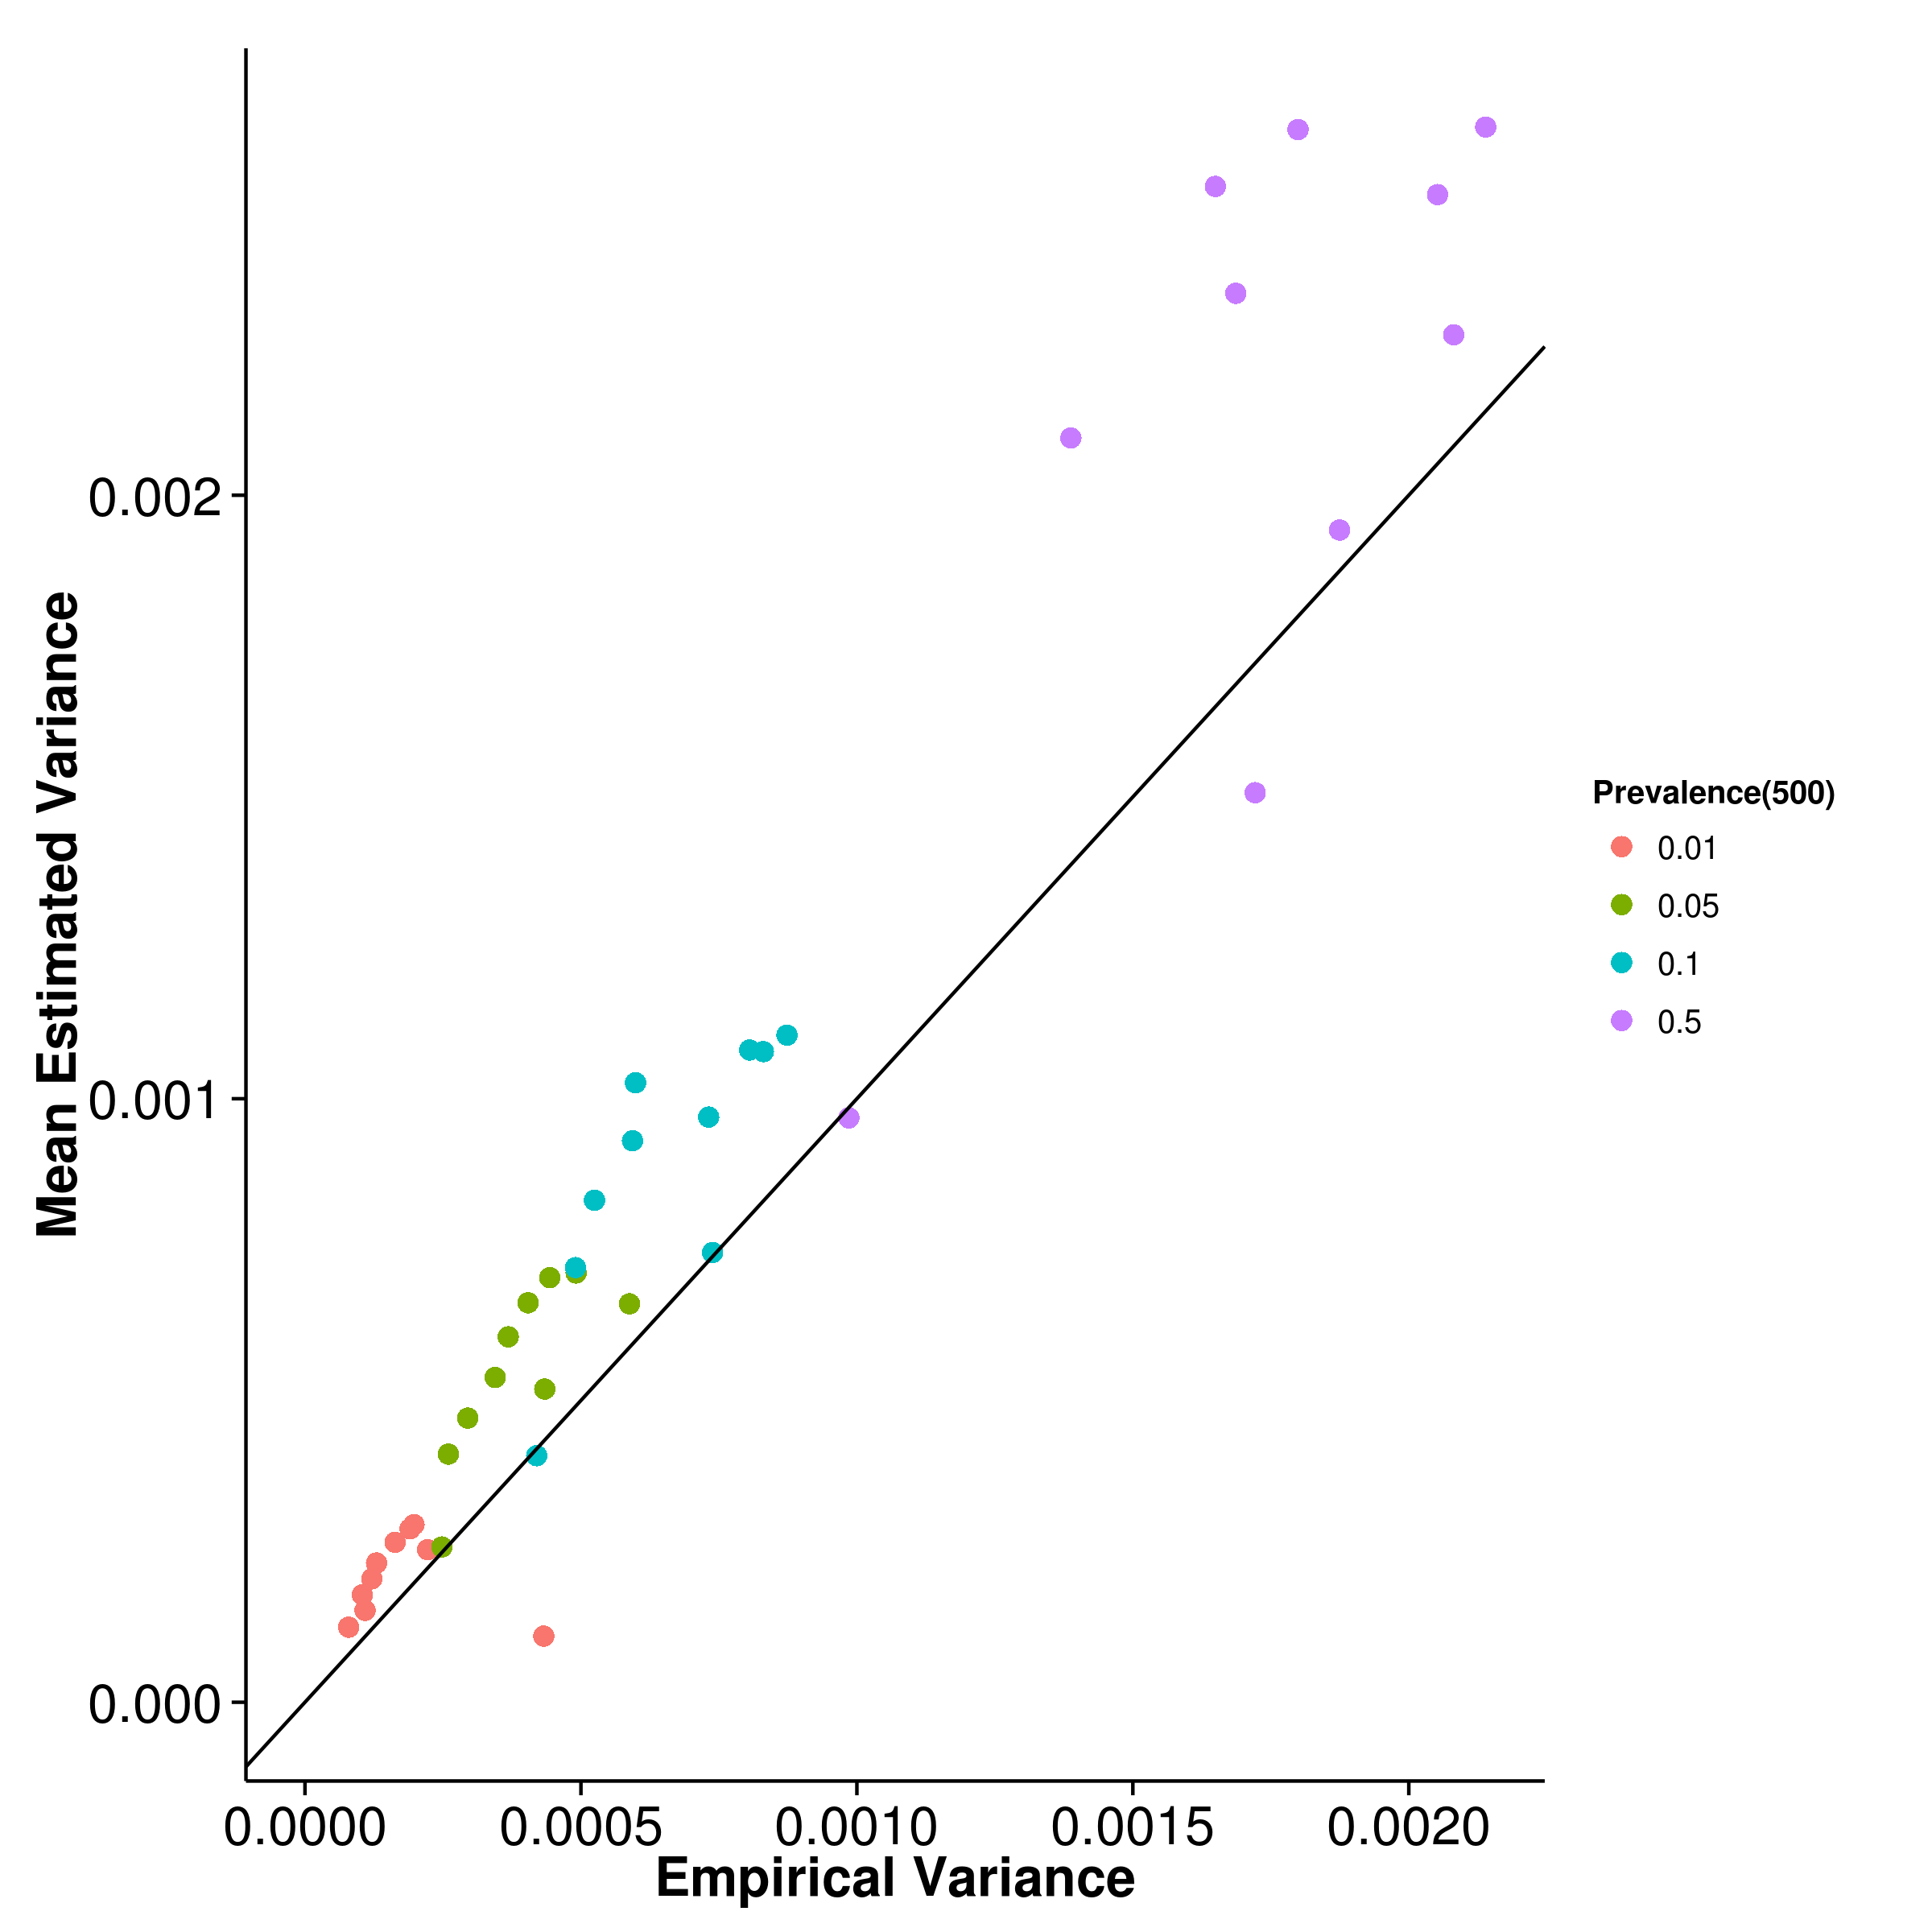
\includegraphics{figure/he_summary/cc_500c/gcta_CC_Rand_sdCom.png}}
				\label{fig:gctaCC500RandVarCom}
			}\\
			\subfloat[LDSC with fix intercept]{
				\scalebox{.4}{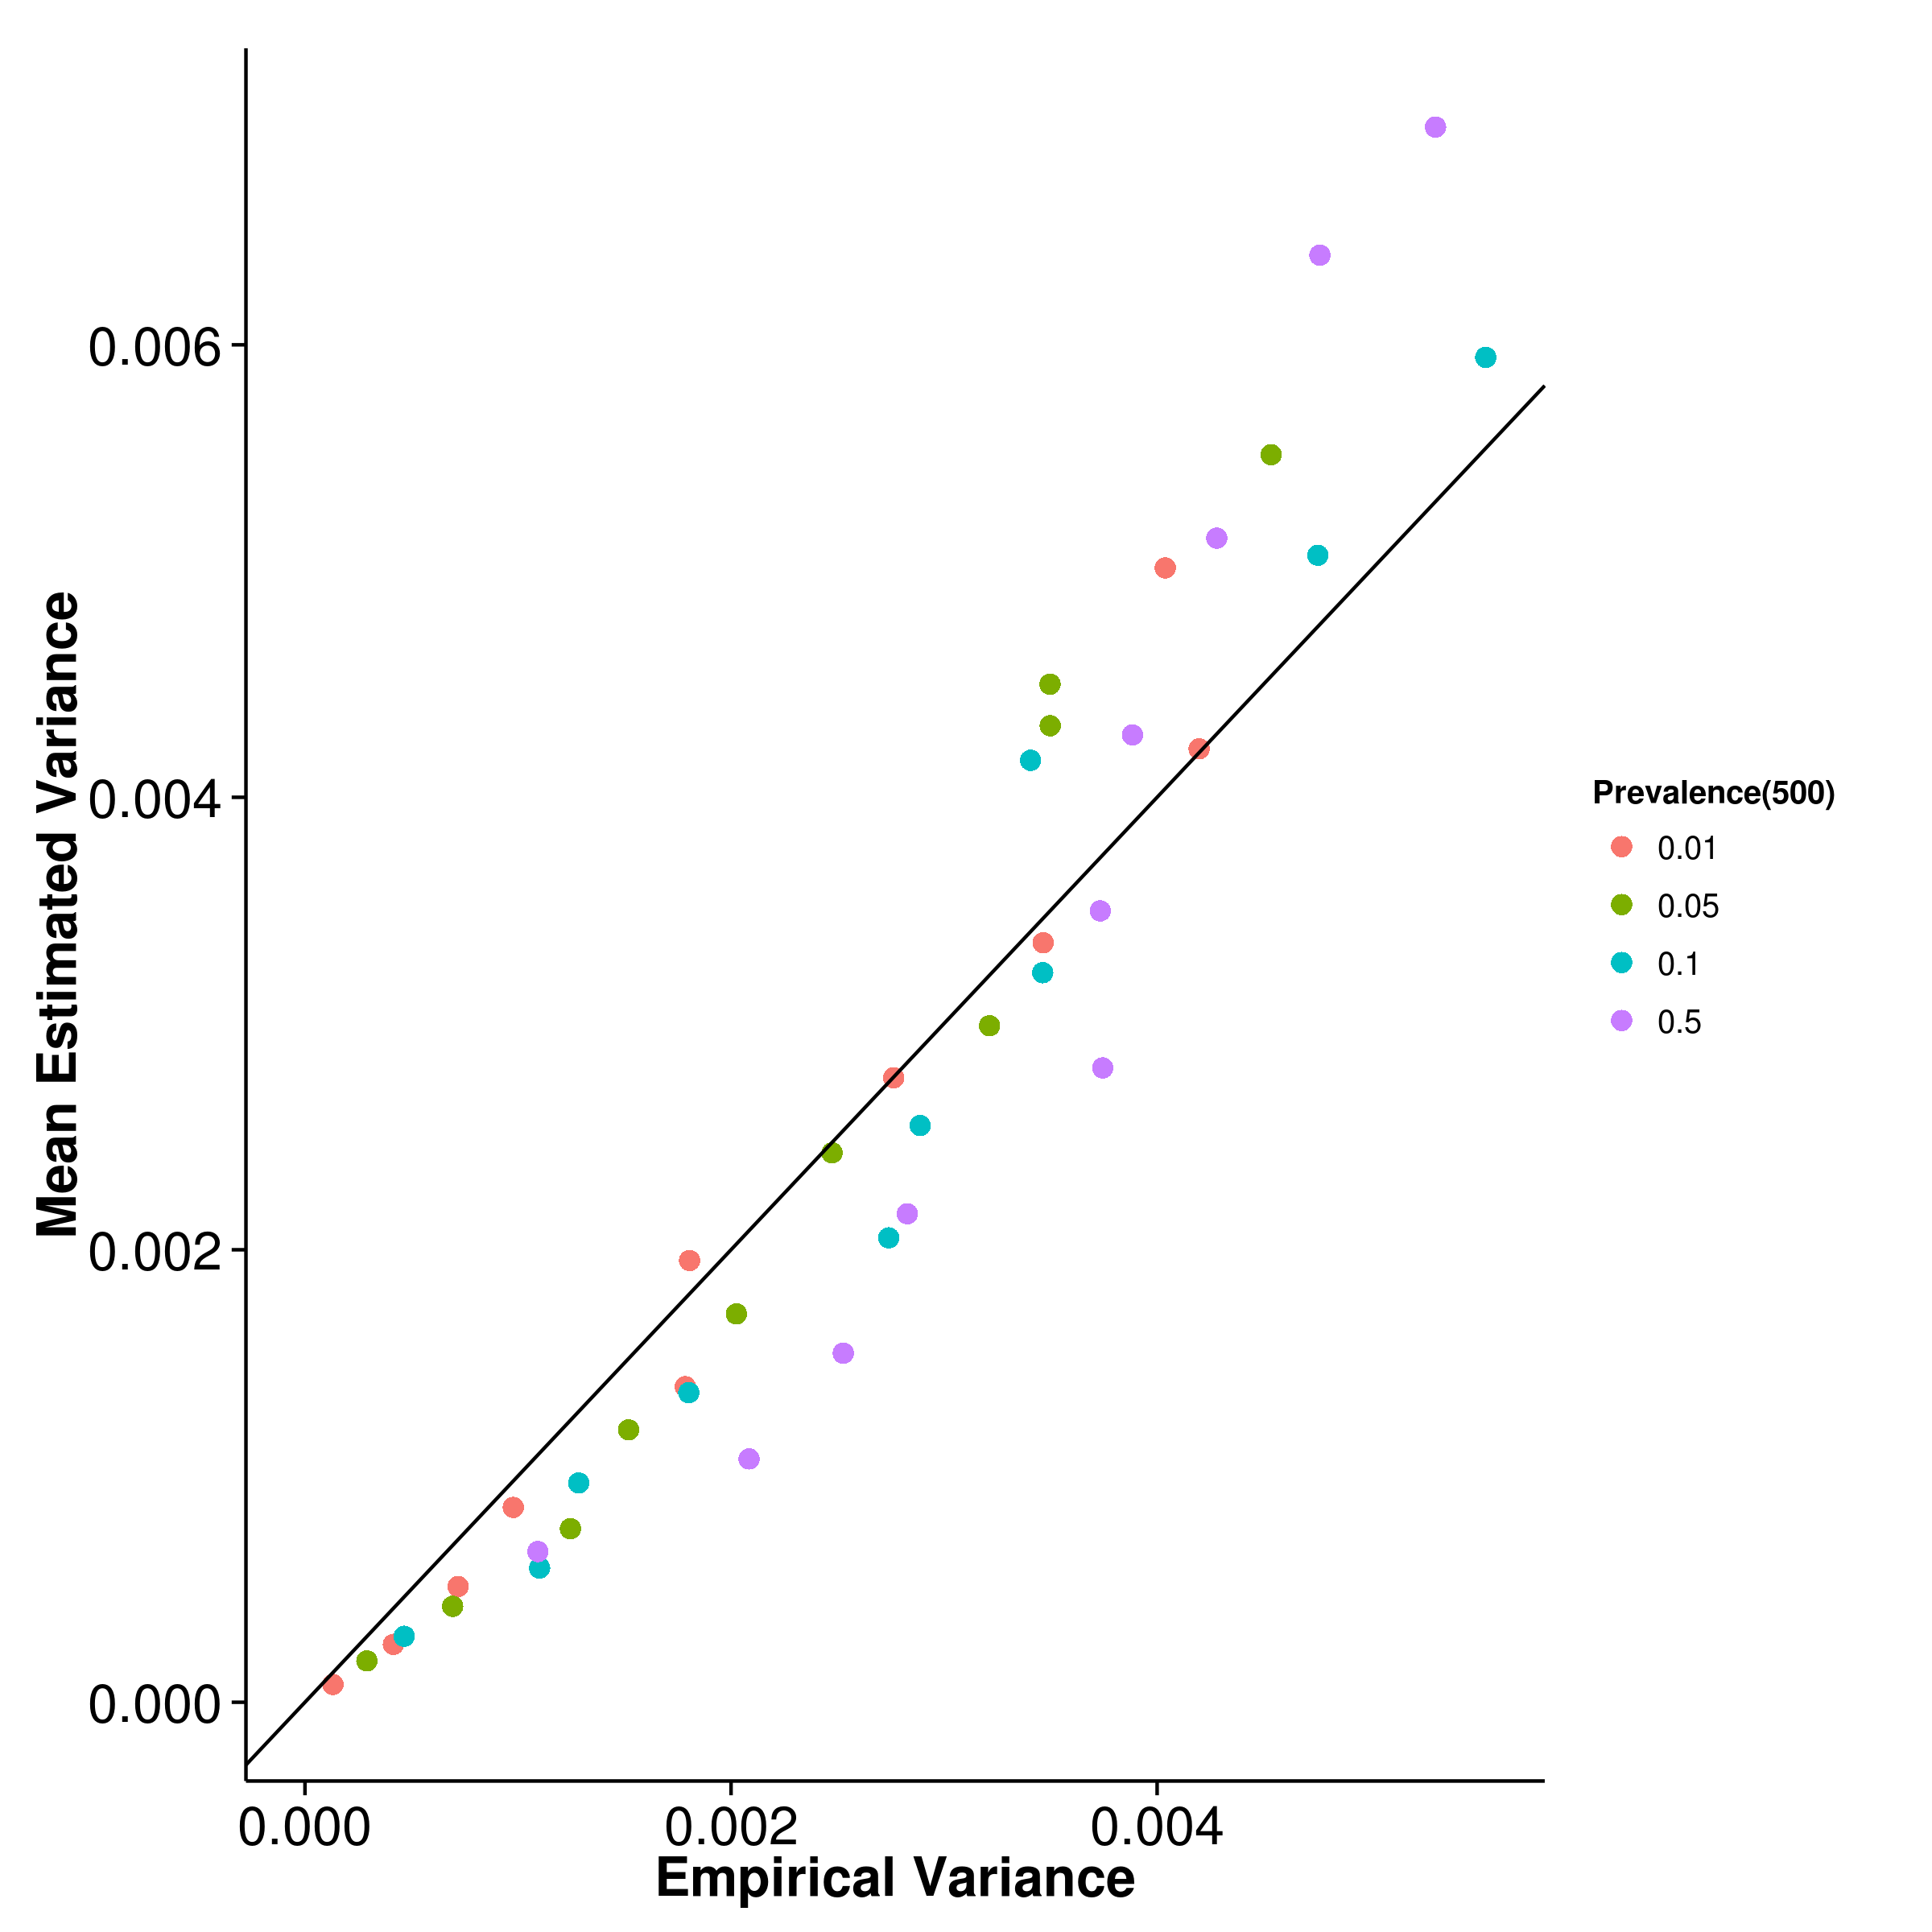
\includegraphics{figure/he_summary/cc_500c/ldsc_CC_Rand_sdCom.png}}
				\label{fig:ldscCC500RandVarCom}
			}
			\subfloat[LDSC with intercept estimation]{
				
				\scalebox{.4}{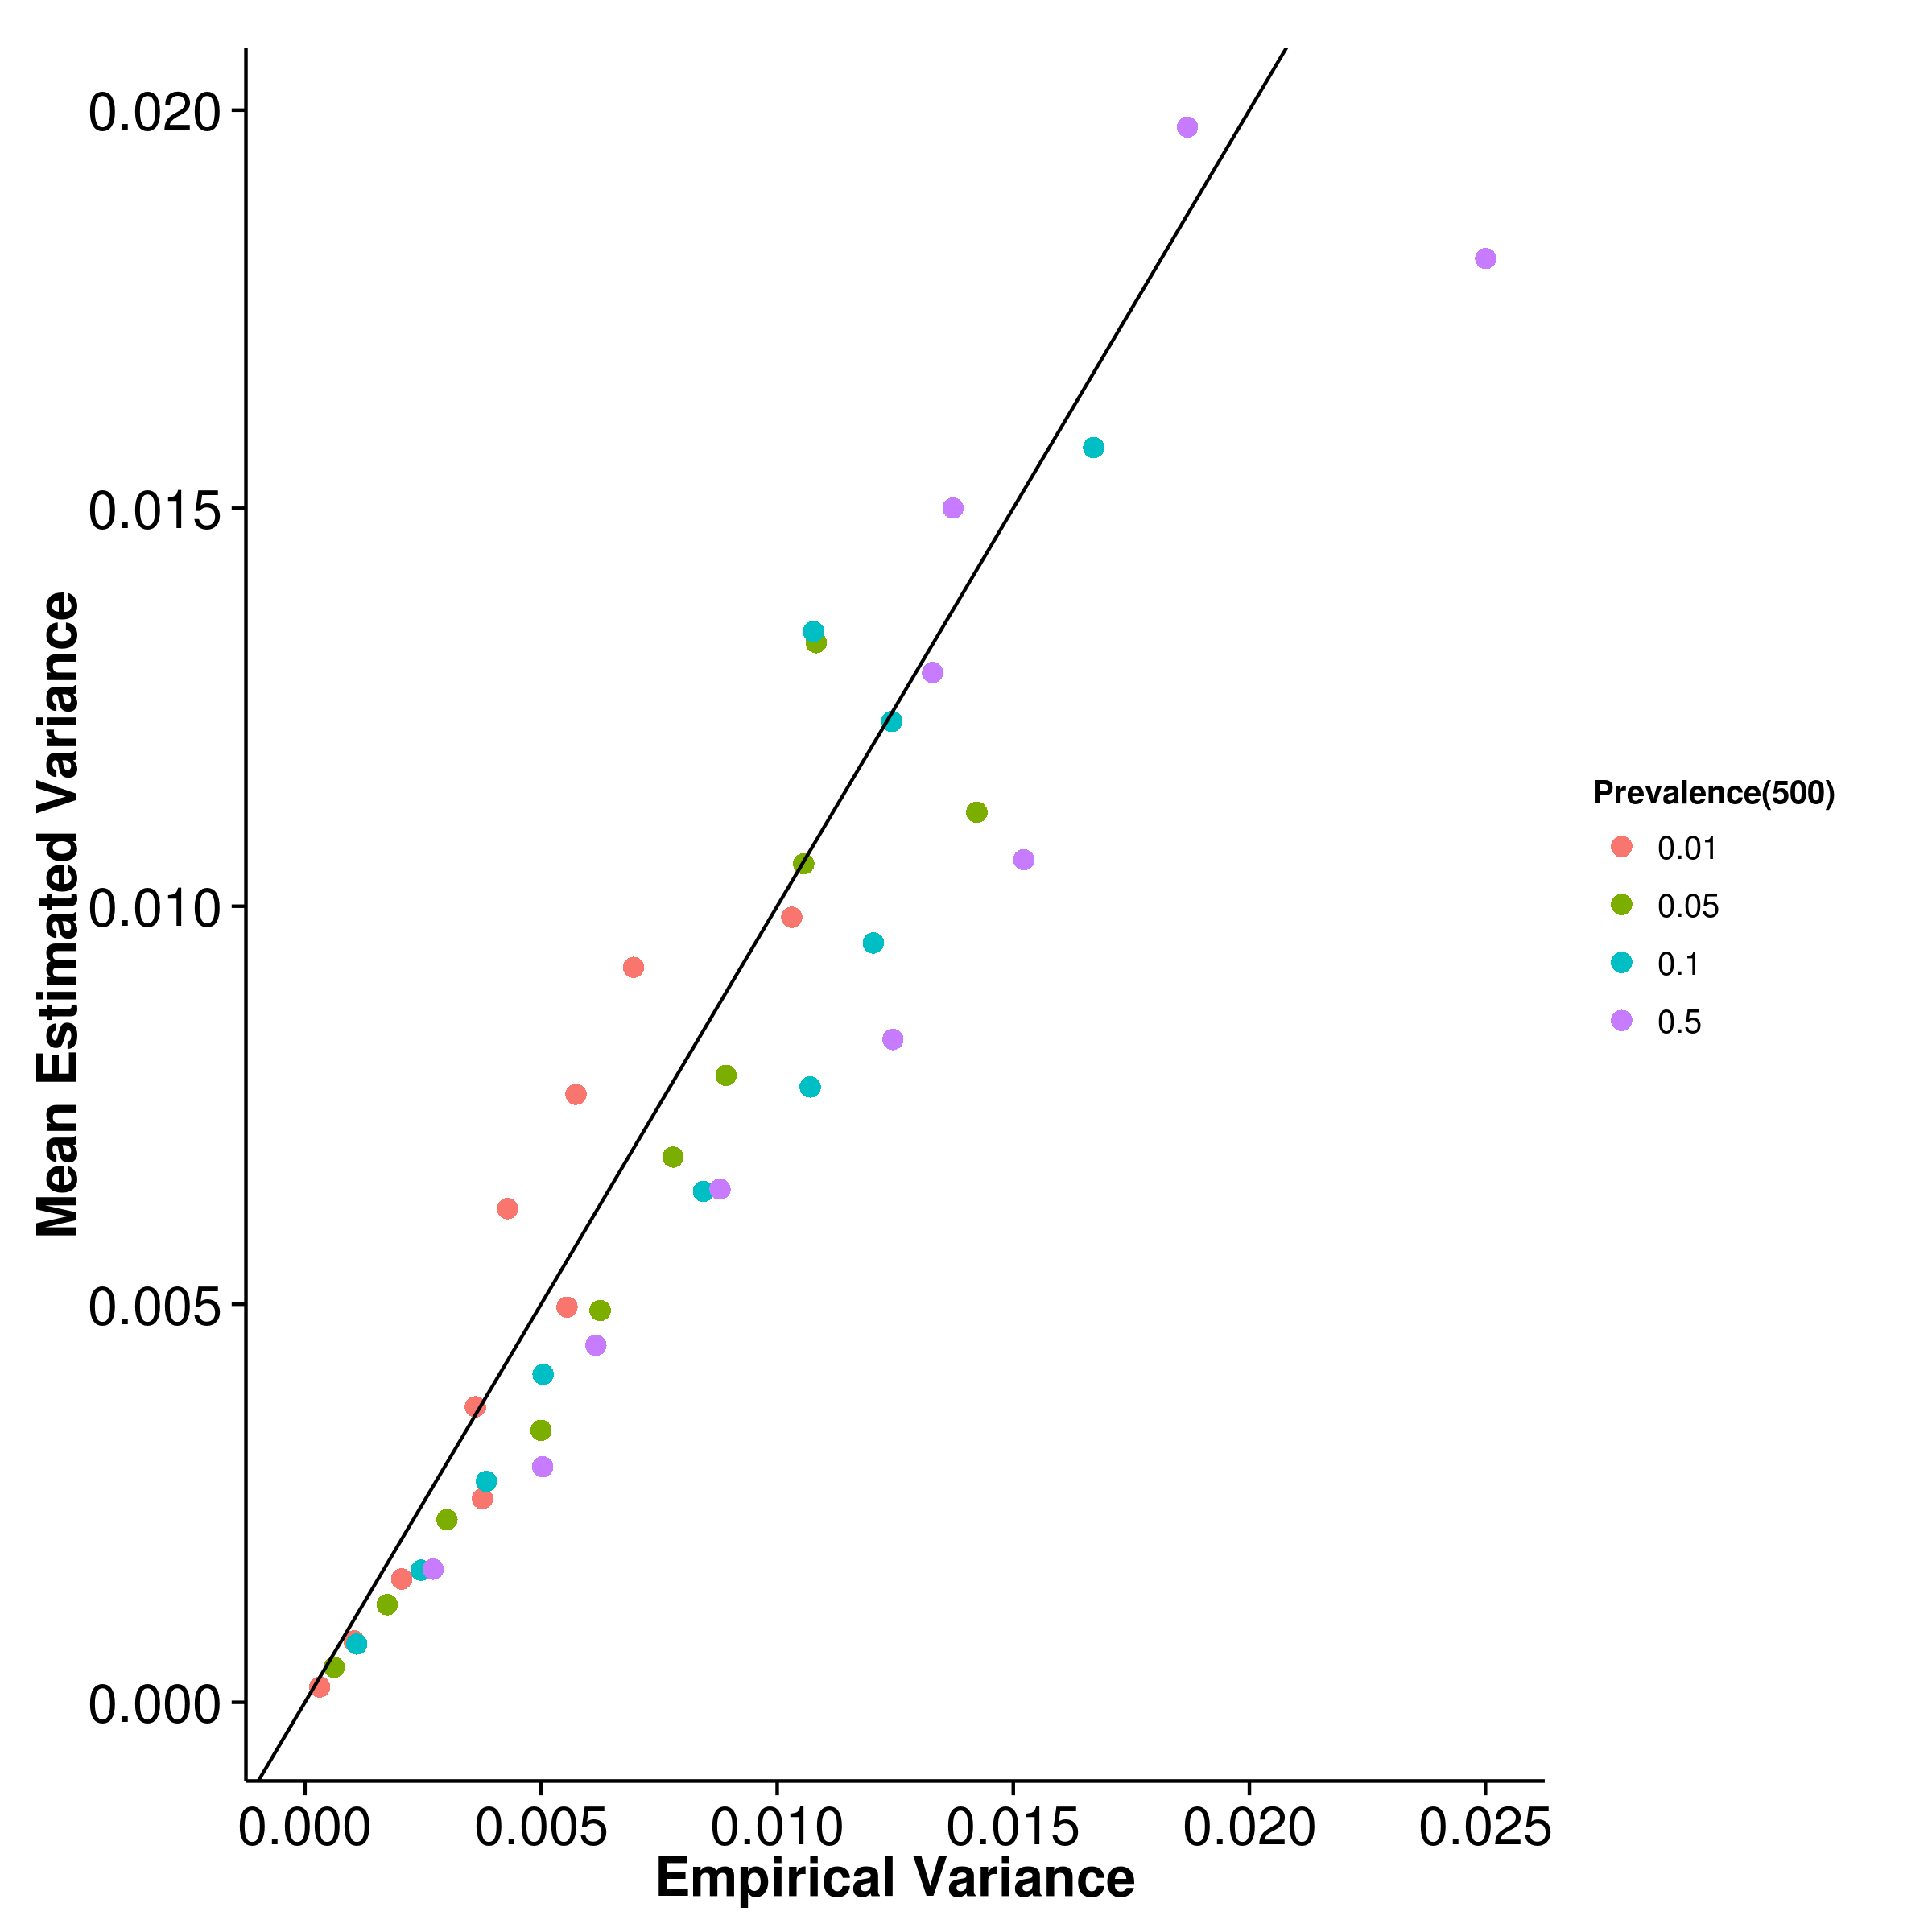
\includegraphics{figure/he_summary/cc_500c/ldscIn_CC_Rand_sdCom.png}}
				\label{fig:ldscInCC500RandVarCom}
			}
			\caption[Estimation of Variance in Case Control Simulation (500 Causal)]
			{Estimated variance of results from case control simulation with random effect size simulation when compared to empirical variance when 500 causal \glspl{SNP} was simulated.
				When the trait contains 500 causal \glspl{SNP}, \gls{ldsc} begins to provide a good estimation of its own empirical variance both with and without intercept estimation. 
				On the other hand, \gls{shrek}'s estimation of its own empirical variance remains consistently lower than the true empirical variance.
			} 
			\label{fig:CC500RandVarCom}
		\end{figure}